%!TeX root=../carlo_master.tex
\chapter{Sensitivity to estimation misspecification across K}\label{sec:misspec_sensitivity_K}

The binary and multiclass campaigns of Sections~\ref{sec:binary_experiments} and~\ref{sec:multiclass_experiments} differ on a secondary observation. On cost-matrix objectives, the lead in overall win/tie rate of the best strategy over the bare analytical plug-in rule narrows from $87\%$ versus $69\%$ in the binary setting (Figure~\ref{fig:win-counts-binary-cost}) to $80\%$ versus $69\%$ in the multiclass setting (Figure~\ref{fig:win-counts-multiclass-cost}), i.e.\ from an $18$-point lead to an $11$-point lead. On the non-decomposable maximization metrics, where the analytical rule reduces to argmax-of-probabilities, the comparison narrows from $100\%$ versus $45\%$ (Figure~\ref{fig:win-counts-binary-max}) to $90\%$ versus $62\%$ (Figure~\ref{fig:win-counts-multiclass-max}). The direction is consistent across both objective families: the lead of the best strategy over the analytical rule shrinks as $K$ grows.

There are two candidate explanations. Either the multiclass validation partition carries little exploitable signal, or the analytical Bayes-optimal rule itself becomes more robust to distributional misspecification as $K$ grows. We test the second reading with two controlled synthetic experiments and propose a candidate mechanism for it.

\section{Synthetic experiments}\label{sec:misspec_sensitivity_experiments}

Both experiments use closed-form Gaussian class-conditional densities and evaluate the analytical Bayes-optimal rule directly under the perturbed distribution; Monte Carlo enters only to evaluate expectations. They differ in the perturbation: variance scaling (Section~\ref{sec:misspec_sensitivity_variance}) is observable only under an asymmetric cost, while per-class random mean shifts (Section~\ref{sec:misspec_sensitivity_meanshift}) break the argmax-invariance and reproduce the K-monotone ordering under both symmetric and asymmetric cost.

\subsection{Variance scaling}\label{sec:misspec_sensitivity_variance}

Let $\mathbb{P}_1$ denote the reference distribution over $(X, Y) \in \mathbb{R}^2 \times \mathcal{Y}$ in which the class priors are uniform ($\pi_k = 1/K$) and each class-conditional density is isotropic Gaussian, $p_1(x \mid Y{=}k) = \mathcal{N}(\mathbf{m}_k, \sigma^2 \mathbf{I})$ with $\sigma = 1$; it is the identity member of the variance family $\{\mathbb{P}_\lambda\}_{\lambda \geq 1}$ defined next. The feature-space class means $\mathbf{m}_k \in \mathbb{R}^2$ are placed at the vertices of a regular $K$-gon of radius $2$, so the geometric arrangement is rotationally symmetric; at this fixed radius the distance between adjacent class means, $4\sin(\pi/K)$, decreases as $K$ grows.

The misspecified member $\mathbb{P}_\lambda$ shares the means and priors of $\mathbb{P}_1$ but scales every class-conditional density to $p_\lambda(x \mid Y{=}k) = \mathcal{N}(\mathbf{m}_k, \lambda\sigma^2 \mathbf{I})$ for a single variance multiplier $\lambda \geq 1$, with the reference recovered at the identity value $\lambda = 1$. Write $\boldsymbol{\eta}_1(x)$ and $\boldsymbol{\eta}_\lambda(x)$ for the conditional class probabilities induced by $\mathbb{P}_1$ and $\mathbb{P}_\lambda$ at $x$. Here $\boldsymbol{\eta}_1$ plays the role of the misspecified plug-in estimate $\hat{\mathbf{p}}$ and $\boldsymbol{\eta}_\lambda$ the role of the truth $\boldsymbol{\eta}$, so the difference $\boldsymbol{\eta}_\lambda - \boldsymbol{\eta}_1$ is the estimation error $\boldsymbol{\epsilon}$ of Section~\ref{sec:analytical_fragility}.

The misspecified rule applies the Bayes-optimal decision $\delta^*$ from~\eqref{eq:bayes_optimal_delta} to $\boldsymbol{\eta}_1(x)$, equivalent to assuming the variance is $\sigma^2$, while the oracle applies the same $\delta^*$ to $\boldsymbol{\eta}_\lambda(x)$. Figure~\ref{fig:misspec-sensitivity-setup-geometry} illustrates the construction at $K = 5$: the assumed unit-variance contours sit inside the larger contours of $\mathbb{P}_\lambda$, and the misspecified rule built for the inner geometry is asked to act on data drawn from the outer one.

\begin{figure}[H]
    \centering
    \documentclass[tikz, border=10pt]{standalone}
\usepackage{tikz}
\usepackage{amsmath}
\usetikzlibrary{calc}

\begin{document}
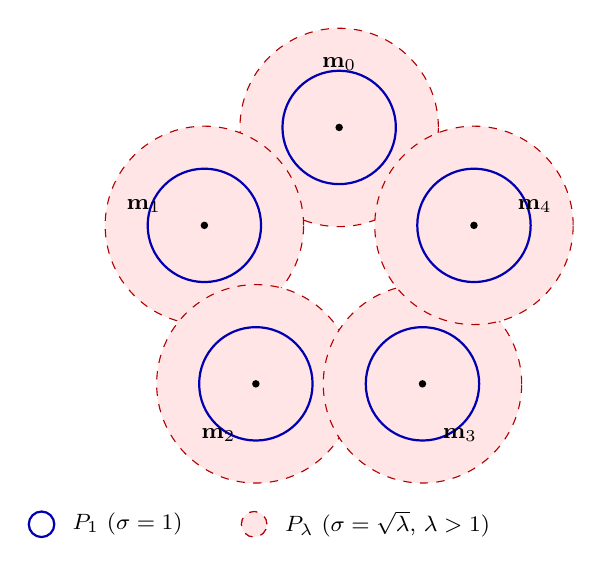
\begin{tikzpicture}[font=\sffamily, scale=0.9]

    % K = 5 class means on a regular K-gon of radius r = 2. mu_0 sits
    % at the top (angle 90 deg); the remaining four vertices are spaced
    % 72 deg apart going counter-clockwise.
    \def\sep{2}
    \def\sigP{0.8}
    \def\sigQ{1.4}

    % Q variance contours, drawn first so the P0 rings sit on top.
    \foreach \i in {0,1,2,3,4} {
        \pgfmathsetmacro{\angle}{90 + 72 * \i}
        \pgfmathsetmacro{\xc}{\sep*cos(\angle)}
        \pgfmathsetmacro{\yc}{\sep*sin(\angle)}
        \fill[red!10] (\xc,\yc) circle (\sigQ);
        \draw[red!70!black, dashed, thin] (\xc,\yc) circle (\sigQ);
    }

    % P0 variance contours plus class-mean dots.
    \foreach \i in {0,1,2,3,4} {
        \pgfmathsetmacro{\angle}{90 + 72 * \i}
        \pgfmathsetmacro{\xc}{\sep*cos(\angle)}
        \pgfmathsetmacro{\yc}{\sep*sin(\angle)}
        \draw[blue!70!black, thick] (\xc,\yc) circle (\sigP);
        \fill[black] (\xc,\yc) circle (1.5pt);
        \pgfmathsetmacro{\lxc}{1.45*\xc}
        \pgfmathsetmacro{\lyc}{1.45*\yc}
        \node[font=\footnotesize] at (\lxc,\lyc) {$\mathbf{m}_{\i}$};
    }

    % Legend.
    \begin{scope}[shift={(-4.2, -3.6)}, font=\footnotesize]
        \draw[blue!70!black, thick] (0,0) circle (0.18);
        \node[anchor=west] at (0.3, 0) {$\mathbb{P}_1$ ($\sigma = 1$)};
        \draw[red!70!black, dashed, thin] (3.0, 0) circle (0.18);
        \fill[red!10] (3.0, 0) circle (0.18);
        \draw[red!70!black, dashed, thin] (3.0, 0) circle (0.18);
        \node[anchor=west] at (3.3, 0) {$\mathbb{P}_\lambda$ ($\sigma = \sqrt{\lambda}$, $\lambda > 1$)};
    \end{scope}

\end{tikzpicture}
\end{document}

    \caption{Variance-scaling perturbation at $K = 5$ in $\mathbb{R}^2$. The class means $\mathbf{m}_k$ sit at the vertices of a regular $K$-gon of radius $2$. Solid blue rings show the $\mathbb{P}_1$ contours at $\sigma = 1$; faded red rings show $\mathbb{P}_\lambda$ contours at $\sigma = \sqrt{\lambda}$ for an example $\lambda > 1$ (here $\lambda \approx 3$). The misspecified rule is built for the inner geometry and applied to data sampled from the outer one.}%
    \label{fig:misspec-sensitivity-setup-geometry}
\end{figure}

The variance multiplier $\lambda$ is the construction's K-independent sweep parameter, so the per-$K$ curves share a common horizontal axis: the per-class KL divergence between $\mathbb{P}_1$ and $\mathbb{P}_\lambda$ equals $(d/2)(\log\lambda + 1/\lambda - 1)$ with $d = 2$, independent of $K$ (Appendix~\ref{app:kl_invariance}). We sweep $17$ log-spaced values of $\lambda$ in $[1, 16]$.

The cost matrix $\mathbf{C}$ is the Asymmetric $10\times$ family from Section~\ref{sec:multiclass_setup}: class $K{-}1$ is designated high-cost so that misclassifying it carries cost $10$, while every other off-diagonal misclassification carries cost $1$. Writing $R_\lambda(h) = \mathbb{E}_{\mathbb{P}_\lambda}[C_{Y, h(X)}]$ for the expected risk of a classifier $h$ under $\mathbb{P}_\lambda$, the oracle classifier is $h^*_\lambda(x) = \delta^*(\boldsymbol{\eta}_\lambda(x))$ and the misspecified classifier is $h^*_1(x) = \delta^*(\boldsymbol{\eta}_1(x))$. We report the relative excess risk,
\begin{equation}
    \frac{R_\lambda(h^*_1) - R_\lambda(h^*_\lambda)}{R_\lambda(h^*_\lambda)},
    \label{eq:misspec_sensitivity_relative_regret}
\end{equation}
which normalises out the baseline difficulty of the cost matrix and is identically zero at $\lambda = 1$ (where the two classifiers coincide).

Expectations are estimated by stratified Monte Carlo. Each task draws $n_{\mathrm{MC}} = 100{,}000$ samples from $\mathbb{P}_\lambda$, evaluates both classifiers on the same samples (shared-sample evaluation cancels most of the Monte Carlo variance in the difference, since the two classifiers agree at every $x$ that is not near a decision boundary), and records both risk estimates. The replicate seed vector is drawn deterministically from a master seed and persisted alongside the run, matching the protocol used by the mean-shift sweep of Section~\ref{sec:misspec_sensitivity_meanshift}. The sweep covers $K \in \{2, 3, 4, 5, 7, 10, 15, 20\}$; the lower endpoint $K = 2$ recovers the binary problem and serves as the bridge to Section~\ref{sec:binary_experiments}.

Figure~\ref{fig:misspec-sensitivity-variance} overlays the eight per-$K$ curves on a single panel. All curves anchor near zero and grow with $\lambda$. The ordering is monotone in $K$ across the bulk of the sweep: at every fixed $\lambda$ above the Monte Carlo floor the $K = 2$ curve sits highest, $K = 3$ next, and so on down to $K = 20$ at the bottom. Between $K = 2$ and $K = 20$ the relative excess risk differs by a factor of roughly seven to eight across $\lambda \in [1, 16]$.

This K-monotone ordering of relative excess risk is the empirical phenomenon predicted qualitatively by the second reading of the section's opening; Section~\ref{sec:misspec_sensitivity_mechanism} proposes a candidate geometric mechanism for it.

\begin{figure}[H]
    \centering
    % Auto-generated by experiments.analysis.generate_variance_figure --- do not edit.
% Cost: Asymmetric 10x. Uniform variance perturbation across classes, lambda >= 1.
% Horizontal axis is the variance multiplier lambda.
% Left log-log, right linear; bands are normal-approx 95% CIs (mean +/- 1.96 * SE).
\noindent\begin{tikzpicture}
\begin{groupplot}[
    group style={group size=2 by 1, horizontal sep=1.6cm},
    width=0.46\textwidth, height=6.0cm,
    grid=major, grid style={dotted, gray!40},
    xmode=log,
    tick label style={font=\scriptsize},
    label style={font=\footnotesize},
    title style={font=\footnotesize},
]
\nextgroupplot[
    title={Asymmetric 10x cost},
    xlabel={Variance multiplier $\lambda$},
    ylabel={$(R_\lambda(h^{\ast}_1) - R_\lambda(h^{\ast}_\lambda)) / R_\lambda(h^{\ast}_\lambda)$},
    ymode=log,
    xmin=0.8323, xmax=22.4, ymin=0.000425688, ymax=2.99919,
]
\addplot[name path=lo_log_K2, draw=none, forget plot] coordinates {
        (1.189, 0.0161447)
        (1.414, 0.0718404)
        (1.682, 0.142239)
        (2, 0.231757)
        (2.378, 0.333251)
        (2.828, 0.441629)
        (3.364, 0.563046)
        (4, 0.692213)
        (4.757, 0.836961)
        (5.657, 0.98451)
        (6.727, 1.13795)
        (8, 1.29971)
        (9.514, 1.46486)
        (11.314, 1.6324)
        (13.454, 1.80237)
        (16, 1.97649)
    };
\addplot[name path=hi_log_K2, draw=none, forget plot] coordinates {
        (1.189, 0.0333247)
        (1.414, 0.0884253)
        (1.682, 0.163695)
        (2, 0.250187)
        (2.378, 0.352524)
        (2.828, 0.462834)
        (3.364, 0.589603)
        (4, 0.722949)
        (4.757, 0.865979)
        (5.657, 1.0107)
        (6.727, 1.16066)
        (8, 1.32026)
        (9.514, 1.48627)
        (11.314, 1.65422)
        (13.454, 1.82666)
        (16, 1.99946)
    };
\addplot[color={rgb,255:red,31; green,119; blue,180}, opacity=0.15, forget plot] fill between [of=lo_log_K2 and hi_log_K2];
\addplot[only marks, mark=*, mark size=1.2pt, color={rgb,255:red,31; green,119; blue,180}] coordinates {
        (1.189, 0.0247347)
        (1.414, 0.0801328)
        (1.682, 0.152967)
        (2, 0.240972)
        (2.378, 0.342888)
        (2.828, 0.452231)
        (3.364, 0.576325)
        (4, 0.707581)
        (4.757, 0.85147)
        (5.657, 0.997606)
        (6.727, 1.14931)
        (8, 1.30999)
        (9.514, 1.47557)
        (11.314, 1.64331)
        (13.454, 1.81451)
        (16, 1.98798)
    };
\addplot[color={rgb,255:red,31; green,119; blue,180}, line width=0.55pt, forget plot] coordinates {
        (1.189, 0.0247347)
        (1.414, 0.0801328)
        (1.682, 0.152967)
        (2, 0.240972)
        (2.378, 0.342888)
        (2.828, 0.452231)
        (3.364, 0.576325)
        (4, 0.707581)
        (4.757, 0.85147)
        (5.657, 0.997606)
        (6.727, 1.14931)
        (8, 1.30999)
        (9.514, 1.47557)
        (11.314, 1.64331)
        (13.454, 1.81451)
        (16, 1.98798)
    };
\addplot[name path=lo_log_K3, draw=none, forget plot] coordinates {
        (1.189, 0.0137686)
        (1.414, 0.0552877)
        (1.682, 0.115988)
        (2, 0.195324)
        (2.378, 0.286426)
        (2.828, 0.382433)
        (3.364, 0.490037)
        (4, 0.593463)
        (4.757, 0.708625)
        (5.657, 0.830985)
        (6.727, 0.952376)
        (8, 1.07403)
        (9.514, 1.20365)
        (11.314, 1.32945)
        (13.454, 1.45665)
        (16, 1.5818)
    };
\addplot[name path=hi_log_K3, draw=none, forget plot] coordinates {
        (1.189, 0.0232883)
        (1.414, 0.0648708)
        (1.682, 0.13004)
        (2, 0.214727)
        (2.378, 0.303447)
        (2.828, 0.40297)
        (3.364, 0.512568)
        (4, 0.618329)
        (4.757, 0.730788)
        (5.657, 0.852117)
        (6.727, 0.97242)
        (8, 1.0927)
        (9.514, 1.21752)
        (11.314, 1.34388)
        (13.454, 1.46793)
        (16, 1.59037)
    };
\addplot[color={rgb,255:red,255; green,127; blue,14}, opacity=0.15, forget plot] fill between [of=lo_log_K3 and hi_log_K3];
\addplot[only marks, mark=*, mark size=1.2pt, color={rgb,255:red,255; green,127; blue,14}] coordinates {
        (1.189, 0.0185285)
        (1.414, 0.0600792)
        (1.682, 0.123014)
        (2, 0.205025)
        (2.378, 0.294936)
        (2.828, 0.392701)
        (3.364, 0.501303)
        (4, 0.605896)
        (4.757, 0.719706)
        (5.657, 0.841551)
        (6.727, 0.962398)
        (8, 1.08336)
        (9.514, 1.21058)
        (11.314, 1.33667)
        (13.454, 1.46229)
        (16, 1.58608)
    };
\addplot[color={rgb,255:red,255; green,127; blue,14}, line width=0.55pt, forget plot] coordinates {
        (1.189, 0.0185285)
        (1.414, 0.0600792)
        (1.682, 0.123014)
        (2, 0.205025)
        (2.378, 0.294936)
        (2.828, 0.392701)
        (3.364, 0.501303)
        (4, 0.605896)
        (4.757, 0.719706)
        (5.657, 0.841551)
        (6.727, 0.962398)
        (8, 1.08336)
        (9.514, 1.21058)
        (11.314, 1.33667)
        (13.454, 1.46229)
        (16, 1.58608)
    };
\addplot[name path=lo_log_K4, draw=none, forget plot] coordinates {
        (1.189, 0.00786415)
        (1.414, 0.0468163)
        (1.682, 0.103907)
        (2, 0.175578)
        (2.378, 0.251519)
        (2.828, 0.339396)
        (3.364, 0.432449)
        (4, 0.526692)
        (4.757, 0.622574)
        (5.657, 0.719398)
        (6.727, 0.818424)
        (8, 0.916216)
        (9.514, 1.01238)
        (11.314, 1.10722)
        (13.454, 1.19747)
        (16, 1.28595)
    };
\addplot[name path=hi_log_K4, draw=none, forget plot] coordinates {
        (1.189, 0.0164744)
        (1.414, 0.0522307)
        (1.682, 0.114793)
        (2, 0.187296)
        (2.378, 0.266792)
        (2.828, 0.352795)
        (3.364, 0.443914)
        (4, 0.542168)
        (4.757, 0.637706)
        (5.657, 0.734813)
        (6.727, 0.831237)
        (8, 0.929232)
        (9.514, 1.02673)
        (11.314, 1.12098)
        (13.454, 1.21126)
        (16, 1.30044)
    };
\addplot[color={rgb,255:red,44; green,160; blue,44}, opacity=0.15, forget plot] fill between [of=lo_log_K4 and hi_log_K4];
\addplot[only marks, mark=*, mark size=1.2pt, color={rgb,255:red,44; green,160; blue,44}] coordinates {
        (1.189, 0.0121693)
        (1.414, 0.0495235)
        (1.682, 0.10935)
        (2, 0.181437)
        (2.378, 0.259155)
        (2.828, 0.346095)
        (3.364, 0.438182)
        (4, 0.53443)
        (4.757, 0.63014)
        (5.657, 0.727105)
        (6.727, 0.82483)
        (8, 0.922724)
        (9.514, 1.01956)
        (11.314, 1.1141)
        (13.454, 1.20437)
        (16, 1.29319)
    };
\addplot[color={rgb,255:red,44; green,160; blue,44}, line width=0.55pt, forget plot] coordinates {
        (1.189, 0.0121693)
        (1.414, 0.0495235)
        (1.682, 0.10935)
        (2, 0.181437)
        (2.378, 0.259155)
        (2.828, 0.346095)
        (3.364, 0.438182)
        (4, 0.53443)
        (4.757, 0.63014)
        (5.657, 0.727105)
        (6.727, 0.82483)
        (8, 0.922724)
        (9.514, 1.01956)
        (11.314, 1.1141)
        (13.454, 1.20437)
        (16, 1.29319)
    };
\addplot[name path=lo_log_K5, draw=none, forget plot] coordinates {
        (1.189, 0.00858714)
        (1.414, 0.0412982)
        (1.682, 0.0908124)
        (2, 0.153464)
        (2.378, 0.220724)
        (2.828, 0.296552)
        (3.364, 0.377461)
        (4, 0.457546)
        (4.757, 0.538286)
        (5.657, 0.618597)
        (6.727, 0.697442)
        (8, 0.773356)
        (9.514, 0.848852)
        (11.314, 0.924177)
        (13.454, 0.995903)
        (16, 1.06329)
    };
\addplot[name path=hi_log_K5, draw=none, forget plot] coordinates {
        (1.189, 0.0134082)
        (1.414, 0.0484077)
        (1.682, 0.0977084)
        (2, 0.163215)
        (2.378, 0.233467)
        (2.828, 0.305662)
        (3.364, 0.386235)
        (4, 0.465198)
        (4.757, 0.545995)
        (5.657, 0.62696)
        (6.727, 0.707023)
        (8, 0.782956)
        (9.514, 0.859622)
        (11.314, 0.934936)
        (13.454, 1.00517)
        (16, 1.07274)
    };
\addplot[color={rgb,255:red,214; green,39; blue,40}, opacity=0.15, forget plot] fill between [of=lo_log_K5 and hi_log_K5];
\addplot[only marks, mark=*, mark size=1.2pt, color={rgb,255:red,214; green,39; blue,40}] coordinates {
        (1.189, 0.0109977)
        (1.414, 0.044853)
        (1.682, 0.0942604)
        (2, 0.15834)
        (2.378, 0.227096)
        (2.828, 0.301107)
        (3.364, 0.381848)
        (4, 0.461372)
        (4.757, 0.54214)
        (5.657, 0.622778)
        (6.727, 0.702232)
        (8, 0.778156)
        (9.514, 0.854237)
        (11.314, 0.929557)
        (13.454, 1.00054)
        (16, 1.06801)
    };
\addplot[color={rgb,255:red,214; green,39; blue,40}, line width=0.55pt, forget plot] coordinates {
        (1.189, 0.0109977)
        (1.414, 0.044853)
        (1.682, 0.0942604)
        (2, 0.15834)
        (2.378, 0.227096)
        (2.828, 0.301107)
        (3.364, 0.381848)
        (4, 0.461372)
        (4.757, 0.54214)
        (5.657, 0.622778)
        (6.727, 0.702232)
        (8, 0.778156)
        (9.514, 0.854237)
        (11.314, 0.929557)
        (13.454, 1.00054)
        (16, 1.06801)
    };
\addplot[name path=lo_log_K7, draw=none, forget plot] coordinates {
        (1.189, 0.00489146)
        (1.414, 0.0256547)
        (1.682, 0.0620802)
        (2, 0.106804)
        (2.378, 0.156521)
        (2.828, 0.211665)
        (3.364, 0.270368)
        (4, 0.329369)
        (4.757, 0.385826)
        (5.657, 0.444772)
        (6.727, 0.505012)
        (8, 0.561215)
        (9.514, 0.616402)
        (11.314, 0.67075)
        (13.454, 0.723249)
        (16, 0.773113)
    };
\addplot[name path=hi_log_K7, draw=none, forget plot] coordinates {
        (1.189, 0.0090175)
        (1.414, 0.0318048)
        (1.682, 0.0671157)
        (2, 0.112398)
        (2.378, 0.162664)
        (2.828, 0.218827)
        (3.364, 0.276874)
        (4, 0.335041)
        (4.757, 0.393183)
        (5.657, 0.454228)
        (6.727, 0.51215)
        (8, 0.570211)
        (9.514, 0.623927)
        (11.314, 0.67861)
        (13.454, 0.730012)
        (16, 0.778521)
    };
\addplot[color={rgb,255:red,148; green,103; blue,189}, opacity=0.15, forget plot] fill between [of=lo_log_K7 and hi_log_K7];
\addplot[only marks, mark=*, mark size=1.2pt, color={rgb,255:red,148; green,103; blue,189}] coordinates {
        (1.189, 0.00695448)
        (1.414, 0.0287297)
        (1.682, 0.064598)
        (2, 0.109601)
        (2.378, 0.159592)
        (2.828, 0.215246)
        (3.364, 0.273621)
        (4, 0.332205)
        (4.757, 0.389504)
        (5.657, 0.4495)
        (6.727, 0.508581)
        (8, 0.565713)
        (9.514, 0.620165)
        (11.314, 0.67468)
        (13.454, 0.72663)
        (16, 0.775817)
    };
\addplot[color={rgb,255:red,148; green,103; blue,189}, line width=0.55pt, forget plot] coordinates {
        (1.189, 0.00695448)
        (1.414, 0.0287297)
        (1.682, 0.064598)
        (2, 0.109601)
        (2.378, 0.159592)
        (2.828, 0.215246)
        (3.364, 0.273621)
        (4, 0.332205)
        (4.757, 0.389504)
        (5.657, 0.4495)
        (6.727, 0.508581)
        (8, 0.565713)
        (9.514, 0.620165)
        (11.314, 0.67468)
        (13.454, 0.72663)
        (16, 0.775817)
    };
\addplot[name path=lo_log_K10, draw=none, forget plot] coordinates {
        (1.189, 0.00241518)
        (1.414, 0.0161753)
        (1.682, 0.0360415)
        (2, 0.0636871)
        (2.378, 0.0957237)
        (2.828, 0.133838)
        (3.364, 0.173433)
        (4, 0.214331)
        (4.757, 0.256292)
        (5.657, 0.298534)
        (6.727, 0.339362)
        (8, 0.379891)
        (9.514, 0.418268)
        (11.314, 0.455481)
        (13.454, 0.491666)
        (16, 0.526482)
    };
\addplot[name path=hi_log_K10, draw=none, forget plot] coordinates {
        (1.189, 0.00459898)
        (1.414, 0.0181741)
        (1.682, 0.0393009)
        (2, 0.0686597)
        (2.378, 0.102639)
        (2.828, 0.140313)
        (3.364, 0.180654)
        (4, 0.219588)
        (4.757, 0.260894)
        (5.657, 0.302297)
        (6.727, 0.342851)
        (8, 0.382769)
        (9.514, 0.422214)
        (11.314, 0.460574)
        (13.454, 0.496621)
        (16, 0.530226)
    };
\addplot[color={rgb,255:red,140; green,86; blue,75}, opacity=0.15, forget plot] fill between [of=lo_log_K10 and hi_log_K10];
\addplot[only marks, mark=*, mark size=1.2pt, color={rgb,255:red,140; green,86; blue,75}] coordinates {
        (1.189, 0.00350708)
        (1.414, 0.0171747)
        (1.682, 0.0376712)
        (2, 0.0661734)
        (2.378, 0.0991812)
        (2.828, 0.137075)
        (3.364, 0.177044)
        (4, 0.216959)
        (4.757, 0.258593)
        (5.657, 0.300416)
        (6.727, 0.341107)
        (8, 0.38133)
        (9.514, 0.420241)
        (11.314, 0.458028)
        (13.454, 0.494143)
        (16, 0.528354)
    };
\addplot[color={rgb,255:red,140; green,86; blue,75}, line width=0.55pt, forget plot] coordinates {
        (1.189, 0.00350708)
        (1.414, 0.0171747)
        (1.682, 0.0376712)
        (2, 0.0661734)
        (2.378, 0.0991812)
        (2.828, 0.137075)
        (3.364, 0.177044)
        (4, 0.216959)
        (4.757, 0.258593)
        (5.657, 0.300416)
        (6.727, 0.341107)
        (8, 0.38133)
        (9.514, 0.420241)
        (11.314, 0.458028)
        (13.454, 0.494143)
        (16, 0.528354)
    };
\addplot[name path=lo_log_K15, draw=none, forget plot] coordinates {
        (1.189, 0.001182)
        (1.414, 0.00862062)
        (1.682, 0.0232245)
        (2, 0.0412677)
        (2.378, 0.0615452)
        (2.828, 0.0847089)
        (3.364, 0.109374)
        (4, 0.135708)
        (4.757, 0.161873)
        (5.657, 0.189942)
        (6.727, 0.214806)
        (8, 0.23984)
        (9.514, 0.263725)
        (11.314, 0.28837)
        (13.454, 0.312157)
        (16, 0.335172)
    };
\addplot[name path=hi_log_K15, draw=none, forget plot] coordinates {
        (1.189, 0.00314398)
        (1.414, 0.012143)
        (1.682, 0.0258598)
        (2, 0.0446189)
        (2.378, 0.0664429)
        (2.828, 0.0901067)
        (3.364, 0.114541)
        (4, 0.140388)
        (4.757, 0.167171)
        (5.657, 0.192335)
        (6.727, 0.218389)
        (8, 0.244384)
        (9.514, 0.270009)
        (11.314, 0.29453)
        (13.454, 0.318543)
        (16, 0.340795)
    };
\addplot[color={rgb,255:red,227; green,119; blue,194}, opacity=0.15, forget plot] fill between [of=lo_log_K15 and hi_log_K15];
\addplot[only marks, mark=*, mark size=1.2pt, color={rgb,255:red,227; green,119; blue,194}] coordinates {
        (1.189, 0.00216299)
        (1.414, 0.0103818)
        (1.682, 0.0245422)
        (2, 0.0429433)
        (2.378, 0.0639941)
        (2.828, 0.0874078)
        (3.364, 0.111958)
        (4, 0.138048)
        (4.757, 0.164522)
        (5.657, 0.191139)
        (6.727, 0.216598)
        (8, 0.242112)
        (9.514, 0.266867)
        (11.314, 0.29145)
        (13.454, 0.31535)
        (16, 0.337984)
    };
\addplot[color={rgb,255:red,227; green,119; blue,194}, line width=0.55pt, forget plot] coordinates {
        (1.189, 0.00216299)
        (1.414, 0.0103818)
        (1.682, 0.0245422)
        (2, 0.0429433)
        (2.378, 0.0639941)
        (2.828, 0.0874078)
        (3.364, 0.111958)
        (4, 0.138048)
        (4.757, 0.164522)
        (5.657, 0.191139)
        (6.727, 0.216598)
        (8, 0.242112)
        (9.514, 0.266867)
        (11.314, 0.29145)
        (13.454, 0.31535)
        (16, 0.337984)
    };
\addplot[name path=lo_log_K20, draw=none, forget plot] coordinates {
        (1.189, 0.0003523)
        (1.414, 0.00614175)
        (1.682, 0.0162756)
        (2, 0.0286209)
        (2.378, 0.0437608)
        (2.828, 0.0615339)
        (3.364, 0.0802796)
        (4, 0.0996629)
        (4.757, 0.118941)
        (5.657, 0.139655)
        (6.727, 0.158926)
        (8, 0.177475)
        (9.514, 0.196231)
        (11.314, 0.21439)
        (13.454, 0.23227)
        (16, 0.248269)
    };
\addplot[name path=hi_log_K20, draw=none, forget plot] coordinates {
        (1.189, 0.00248562)
        (1.414, 0.00882633)
        (1.682, 0.0184819)
        (2, 0.0318147)
        (2.378, 0.0482381)
        (2.828, 0.0651807)
        (3.364, 0.0842073)
        (4, 0.103315)
        (4.757, 0.122889)
        (5.657, 0.142877)
        (6.727, 0.161536)
        (8, 0.181019)
        (9.514, 0.199929)
        (11.314, 0.218523)
        (13.454, 0.236528)
        (16, 0.252079)
    };
\addplot[color={rgb,255:red,127; green,127; blue,127}, opacity=0.15, forget plot] fill between [of=lo_log_K20 and hi_log_K20];
\addplot[only marks, mark=*, mark size=1.2pt, color={rgb,255:red,127; green,127; blue,127}] coordinates {
        (1.189, 0.00141896)
        (1.414, 0.00748404)
        (1.682, 0.0173788)
        (2, 0.0302178)
        (2.378, 0.0459995)
        (2.828, 0.0633573)
        (3.364, 0.0822435)
        (4, 0.101489)
        (4.757, 0.120915)
        (5.657, 0.141266)
        (6.727, 0.160231)
        (8, 0.179247)
        (9.514, 0.19808)
        (11.314, 0.216457)
        (13.454, 0.234399)
        (16, 0.250174)
    };
\addplot[color={rgb,255:red,127; green,127; blue,127}, line width=0.55pt, forget plot] coordinates {
        (1.189, 0.00141896)
        (1.414, 0.00748404)
        (1.682, 0.0173788)
        (2, 0.0302178)
        (2.378, 0.0459995)
        (2.828, 0.0633573)
        (3.364, 0.0822435)
        (4, 0.101489)
        (4.757, 0.120915)
        (5.657, 0.141266)
        (6.727, 0.160231)
        (8, 0.179247)
        (9.514, 0.19808)
        (11.314, 0.216457)
        (13.454, 0.234399)
        (16, 0.250174)
    };
\nextgroupplot[
    title={Asymmetric 10x cost},
    xlabel={Variance multiplier $\lambda$},
    ymode=normal,
    legend style={font=\scriptsize, fill opacity=0.85, draw=none, at={(0.02,0.98)}, anchor=north west},
    legend cell align=left,
    xmin=0.7, xmax=22.4, ymin=0, ymax=2.09943,
]
\addplot[name path=lo_lin_K2, draw=none, forget plot] coordinates {
        (1, 0)
        (1.189, 0.0161447)
        (1.414, 0.0718404)
        (1.682, 0.142239)
        (2, 0.231757)
        (2.378, 0.333251)
        (2.828, 0.441629)
        (3.364, 0.563046)
        (4, 0.692213)
        (4.757, 0.836961)
        (5.657, 0.98451)
        (6.727, 1.13795)
        (8, 1.29971)
        (9.514, 1.46486)
        (11.314, 1.6324)
        (13.454, 1.80237)
        (16, 1.97649)
    };
\addplot[name path=hi_lin_K2, draw=none, forget plot] coordinates {
        (1, 0)
        (1.189, 0.0333247)
        (1.414, 0.0884253)
        (1.682, 0.163695)
        (2, 0.250187)
        (2.378, 0.352524)
        (2.828, 0.462834)
        (3.364, 0.589603)
        (4, 0.722949)
        (4.757, 0.865979)
        (5.657, 1.0107)
        (6.727, 1.16066)
        (8, 1.32026)
        (9.514, 1.48627)
        (11.314, 1.65422)
        (13.454, 1.82666)
        (16, 1.99946)
    };
\addplot[color={rgb,255:red,31; green,119; blue,180}, opacity=0.15, forget plot] fill between [of=lo_lin_K2 and hi_lin_K2];
\addplot[only marks, mark=*, mark size=1.2pt, color={rgb,255:red,31; green,119; blue,180}] coordinates {
        (1, 0)
        (1.189, 0.0247347)
        (1.414, 0.0801328)
        (1.682, 0.152967)
        (2, 0.240972)
        (2.378, 0.342888)
        (2.828, 0.452231)
        (3.364, 0.576325)
        (4, 0.707581)
        (4.757, 0.85147)
        (5.657, 0.997606)
        (6.727, 1.14931)
        (8, 1.30999)
        (9.514, 1.47557)
        (11.314, 1.64331)
        (13.454, 1.81451)
        (16, 1.98798)
    };
\addplot[color={rgb,255:red,31; green,119; blue,180}, line width=0.55pt, forget plot] coordinates {
        (1, 0)
        (1.189, 0.0247347)
        (1.414, 0.0801328)
        (1.682, 0.152967)
        (2, 0.240972)
        (2.378, 0.342888)
        (2.828, 0.452231)
        (3.364, 0.576325)
        (4, 0.707581)
        (4.757, 0.85147)
        (5.657, 0.997606)
        (6.727, 1.14931)
        (8, 1.30999)
        (9.514, 1.47557)
        (11.314, 1.64331)
        (13.454, 1.81451)
        (16, 1.98798)
    };
\addplot[name path=lo_lin_K3, draw=none, forget plot] coordinates {
        (1, 0)
        (1.189, 0.0137686)
        (1.414, 0.0552877)
        (1.682, 0.115988)
        (2, 0.195324)
        (2.378, 0.286426)
        (2.828, 0.382433)
        (3.364, 0.490037)
        (4, 0.593463)
        (4.757, 0.708625)
        (5.657, 0.830985)
        (6.727, 0.952376)
        (8, 1.07403)
        (9.514, 1.20365)
        (11.314, 1.32945)
        (13.454, 1.45665)
        (16, 1.5818)
    };
\addplot[name path=hi_lin_K3, draw=none, forget plot] coordinates {
        (1, 0)
        (1.189, 0.0232883)
        (1.414, 0.0648708)
        (1.682, 0.13004)
        (2, 0.214727)
        (2.378, 0.303447)
        (2.828, 0.40297)
        (3.364, 0.512568)
        (4, 0.618329)
        (4.757, 0.730788)
        (5.657, 0.852117)
        (6.727, 0.97242)
        (8, 1.0927)
        (9.514, 1.21752)
        (11.314, 1.34388)
        (13.454, 1.46793)
        (16, 1.59037)
    };
\addplot[color={rgb,255:red,255; green,127; blue,14}, opacity=0.15, forget plot] fill between [of=lo_lin_K3 and hi_lin_K3];
\addplot[only marks, mark=*, mark size=1.2pt, color={rgb,255:red,255; green,127; blue,14}] coordinates {
        (1, 0)
        (1.189, 0.0185285)
        (1.414, 0.0600792)
        (1.682, 0.123014)
        (2, 0.205025)
        (2.378, 0.294936)
        (2.828, 0.392701)
        (3.364, 0.501303)
        (4, 0.605896)
        (4.757, 0.719706)
        (5.657, 0.841551)
        (6.727, 0.962398)
        (8, 1.08336)
        (9.514, 1.21058)
        (11.314, 1.33667)
        (13.454, 1.46229)
        (16, 1.58608)
    };
\addplot[color={rgb,255:red,255; green,127; blue,14}, line width=0.55pt, forget plot] coordinates {
        (1, 0)
        (1.189, 0.0185285)
        (1.414, 0.0600792)
        (1.682, 0.123014)
        (2, 0.205025)
        (2.378, 0.294936)
        (2.828, 0.392701)
        (3.364, 0.501303)
        (4, 0.605896)
        (4.757, 0.719706)
        (5.657, 0.841551)
        (6.727, 0.962398)
        (8, 1.08336)
        (9.514, 1.21058)
        (11.314, 1.33667)
        (13.454, 1.46229)
        (16, 1.58608)
    };
\addplot[name path=lo_lin_K4, draw=none, forget plot] coordinates {
        (1, 0)
        (1.189, 0.00786415)
        (1.414, 0.0468163)
        (1.682, 0.103907)
        (2, 0.175578)
        (2.378, 0.251519)
        (2.828, 0.339396)
        (3.364, 0.432449)
        (4, 0.526692)
        (4.757, 0.622574)
        (5.657, 0.719398)
        (6.727, 0.818424)
        (8, 0.916216)
        (9.514, 1.01238)
        (11.314, 1.10722)
        (13.454, 1.19747)
        (16, 1.28595)
    };
\addplot[name path=hi_lin_K4, draw=none, forget plot] coordinates {
        (1, 0)
        (1.189, 0.0164744)
        (1.414, 0.0522307)
        (1.682, 0.114793)
        (2, 0.187296)
        (2.378, 0.266792)
        (2.828, 0.352795)
        (3.364, 0.443914)
        (4, 0.542168)
        (4.757, 0.637706)
        (5.657, 0.734813)
        (6.727, 0.831237)
        (8, 0.929232)
        (9.514, 1.02673)
        (11.314, 1.12098)
        (13.454, 1.21126)
        (16, 1.30044)
    };
\addplot[color={rgb,255:red,44; green,160; blue,44}, opacity=0.15, forget plot] fill between [of=lo_lin_K4 and hi_lin_K4];
\addplot[only marks, mark=*, mark size=1.2pt, color={rgb,255:red,44; green,160; blue,44}] coordinates {
        (1, 0)
        (1.189, 0.0121693)
        (1.414, 0.0495235)
        (1.682, 0.10935)
        (2, 0.181437)
        (2.378, 0.259155)
        (2.828, 0.346095)
        (3.364, 0.438182)
        (4, 0.53443)
        (4.757, 0.63014)
        (5.657, 0.727105)
        (6.727, 0.82483)
        (8, 0.922724)
        (9.514, 1.01956)
        (11.314, 1.1141)
        (13.454, 1.20437)
        (16, 1.29319)
    };
\addplot[color={rgb,255:red,44; green,160; blue,44}, line width=0.55pt, forget plot] coordinates {
        (1, 0)
        (1.189, 0.0121693)
        (1.414, 0.0495235)
        (1.682, 0.10935)
        (2, 0.181437)
        (2.378, 0.259155)
        (2.828, 0.346095)
        (3.364, 0.438182)
        (4, 0.53443)
        (4.757, 0.63014)
        (5.657, 0.727105)
        (6.727, 0.82483)
        (8, 0.922724)
        (9.514, 1.01956)
        (11.314, 1.1141)
        (13.454, 1.20437)
        (16, 1.29319)
    };
\addplot[name path=lo_lin_K5, draw=none, forget plot] coordinates {
        (1, 0)
        (1.189, 0.00858714)
        (1.414, 0.0412982)
        (1.682, 0.0908124)
        (2, 0.153464)
        (2.378, 0.220724)
        (2.828, 0.296552)
        (3.364, 0.377461)
        (4, 0.457546)
        (4.757, 0.538286)
        (5.657, 0.618597)
        (6.727, 0.697442)
        (8, 0.773356)
        (9.514, 0.848852)
        (11.314, 0.924177)
        (13.454, 0.995903)
        (16, 1.06329)
    };
\addplot[name path=hi_lin_K5, draw=none, forget plot] coordinates {
        (1, 0)
        (1.189, 0.0134082)
        (1.414, 0.0484077)
        (1.682, 0.0977084)
        (2, 0.163215)
        (2.378, 0.233467)
        (2.828, 0.305662)
        (3.364, 0.386235)
        (4, 0.465198)
        (4.757, 0.545995)
        (5.657, 0.62696)
        (6.727, 0.707023)
        (8, 0.782956)
        (9.514, 0.859622)
        (11.314, 0.934936)
        (13.454, 1.00517)
        (16, 1.07274)
    };
\addplot[color={rgb,255:red,214; green,39; blue,40}, opacity=0.15, forget plot] fill between [of=lo_lin_K5 and hi_lin_K5];
\addplot[only marks, mark=*, mark size=1.2pt, color={rgb,255:red,214; green,39; blue,40}] coordinates {
        (1, 0)
        (1.189, 0.0109977)
        (1.414, 0.044853)
        (1.682, 0.0942604)
        (2, 0.15834)
        (2.378, 0.227096)
        (2.828, 0.301107)
        (3.364, 0.381848)
        (4, 0.461372)
        (4.757, 0.54214)
        (5.657, 0.622778)
        (6.727, 0.702232)
        (8, 0.778156)
        (9.514, 0.854237)
        (11.314, 0.929557)
        (13.454, 1.00054)
        (16, 1.06801)
    };
\addplot[color={rgb,255:red,214; green,39; blue,40}, line width=0.55pt, forget plot] coordinates {
        (1, 0)
        (1.189, 0.0109977)
        (1.414, 0.044853)
        (1.682, 0.0942604)
        (2, 0.15834)
        (2.378, 0.227096)
        (2.828, 0.301107)
        (3.364, 0.381848)
        (4, 0.461372)
        (4.757, 0.54214)
        (5.657, 0.622778)
        (6.727, 0.702232)
        (8, 0.778156)
        (9.514, 0.854237)
        (11.314, 0.929557)
        (13.454, 1.00054)
        (16, 1.06801)
    };
\addplot[name path=lo_lin_K7, draw=none, forget plot] coordinates {
        (1, 0)
        (1.189, 0.00489146)
        (1.414, 0.0256547)
        (1.682, 0.0620802)
        (2, 0.106804)
        (2.378, 0.156521)
        (2.828, 0.211665)
        (3.364, 0.270368)
        (4, 0.329369)
        (4.757, 0.385826)
        (5.657, 0.444772)
        (6.727, 0.505012)
        (8, 0.561215)
        (9.514, 0.616402)
        (11.314, 0.67075)
        (13.454, 0.723249)
        (16, 0.773113)
    };
\addplot[name path=hi_lin_K7, draw=none, forget plot] coordinates {
        (1, 0)
        (1.189, 0.0090175)
        (1.414, 0.0318048)
        (1.682, 0.0671157)
        (2, 0.112398)
        (2.378, 0.162664)
        (2.828, 0.218827)
        (3.364, 0.276874)
        (4, 0.335041)
        (4.757, 0.393183)
        (5.657, 0.454228)
        (6.727, 0.51215)
        (8, 0.570211)
        (9.514, 0.623927)
        (11.314, 0.67861)
        (13.454, 0.730012)
        (16, 0.778521)
    };
\addplot[color={rgb,255:red,148; green,103; blue,189}, opacity=0.15, forget plot] fill between [of=lo_lin_K7 and hi_lin_K7];
\addplot[only marks, mark=*, mark size=1.2pt, color={rgb,255:red,148; green,103; blue,189}] coordinates {
        (1, 0)
        (1.189, 0.00695448)
        (1.414, 0.0287297)
        (1.682, 0.064598)
        (2, 0.109601)
        (2.378, 0.159592)
        (2.828, 0.215246)
        (3.364, 0.273621)
        (4, 0.332205)
        (4.757, 0.389504)
        (5.657, 0.4495)
        (6.727, 0.508581)
        (8, 0.565713)
        (9.514, 0.620165)
        (11.314, 0.67468)
        (13.454, 0.72663)
        (16, 0.775817)
    };
\addplot[color={rgb,255:red,148; green,103; blue,189}, line width=0.55pt, forget plot] coordinates {
        (1, 0)
        (1.189, 0.00695448)
        (1.414, 0.0287297)
        (1.682, 0.064598)
        (2, 0.109601)
        (2.378, 0.159592)
        (2.828, 0.215246)
        (3.364, 0.273621)
        (4, 0.332205)
        (4.757, 0.389504)
        (5.657, 0.4495)
        (6.727, 0.508581)
        (8, 0.565713)
        (9.514, 0.620165)
        (11.314, 0.67468)
        (13.454, 0.72663)
        (16, 0.775817)
    };
\addplot[name path=lo_lin_K10, draw=none, forget plot] coordinates {
        (1, 0)
        (1.189, 0.00241518)
        (1.414, 0.0161753)
        (1.682, 0.0360415)
        (2, 0.0636871)
        (2.378, 0.0957237)
        (2.828, 0.133838)
        (3.364, 0.173433)
        (4, 0.214331)
        (4.757, 0.256292)
        (5.657, 0.298534)
        (6.727, 0.339362)
        (8, 0.379891)
        (9.514, 0.418268)
        (11.314, 0.455481)
        (13.454, 0.491666)
        (16, 0.526482)
    };
\addplot[name path=hi_lin_K10, draw=none, forget plot] coordinates {
        (1, 0)
        (1.189, 0.00459898)
        (1.414, 0.0181741)
        (1.682, 0.0393009)
        (2, 0.0686597)
        (2.378, 0.102639)
        (2.828, 0.140313)
        (3.364, 0.180654)
        (4, 0.219588)
        (4.757, 0.260894)
        (5.657, 0.302297)
        (6.727, 0.342851)
        (8, 0.382769)
        (9.514, 0.422214)
        (11.314, 0.460574)
        (13.454, 0.496621)
        (16, 0.530226)
    };
\addplot[color={rgb,255:red,140; green,86; blue,75}, opacity=0.15, forget plot] fill between [of=lo_lin_K10 and hi_lin_K10];
\addplot[only marks, mark=*, mark size=1.2pt, color={rgb,255:red,140; green,86; blue,75}] coordinates {
        (1, 0)
        (1.189, 0.00350708)
        (1.414, 0.0171747)
        (1.682, 0.0376712)
        (2, 0.0661734)
        (2.378, 0.0991812)
        (2.828, 0.137075)
        (3.364, 0.177044)
        (4, 0.216959)
        (4.757, 0.258593)
        (5.657, 0.300416)
        (6.727, 0.341107)
        (8, 0.38133)
        (9.514, 0.420241)
        (11.314, 0.458028)
        (13.454, 0.494143)
        (16, 0.528354)
    };
\addplot[color={rgb,255:red,140; green,86; blue,75}, line width=0.55pt, forget plot] coordinates {
        (1, 0)
        (1.189, 0.00350708)
        (1.414, 0.0171747)
        (1.682, 0.0376712)
        (2, 0.0661734)
        (2.378, 0.0991812)
        (2.828, 0.137075)
        (3.364, 0.177044)
        (4, 0.216959)
        (4.757, 0.258593)
        (5.657, 0.300416)
        (6.727, 0.341107)
        (8, 0.38133)
        (9.514, 0.420241)
        (11.314, 0.458028)
        (13.454, 0.494143)
        (16, 0.528354)
    };
\addplot[name path=lo_lin_K15, draw=none, forget plot] coordinates {
        (1, 0)
        (1.189, 0.001182)
        (1.414, 0.00862062)
        (1.682, 0.0232245)
        (2, 0.0412677)
        (2.378, 0.0615452)
        (2.828, 0.0847089)
        (3.364, 0.109374)
        (4, 0.135708)
        (4.757, 0.161873)
        (5.657, 0.189942)
        (6.727, 0.214806)
        (8, 0.23984)
        (9.514, 0.263725)
        (11.314, 0.28837)
        (13.454, 0.312157)
        (16, 0.335172)
    };
\addplot[name path=hi_lin_K15, draw=none, forget plot] coordinates {
        (1, 0)
        (1.189, 0.00314398)
        (1.414, 0.012143)
        (1.682, 0.0258598)
        (2, 0.0446189)
        (2.378, 0.0664429)
        (2.828, 0.0901067)
        (3.364, 0.114541)
        (4, 0.140388)
        (4.757, 0.167171)
        (5.657, 0.192335)
        (6.727, 0.218389)
        (8, 0.244384)
        (9.514, 0.270009)
        (11.314, 0.29453)
        (13.454, 0.318543)
        (16, 0.340795)
    };
\addplot[color={rgb,255:red,227; green,119; blue,194}, opacity=0.15, forget plot] fill between [of=lo_lin_K15 and hi_lin_K15];
\addplot[only marks, mark=*, mark size=1.2pt, color={rgb,255:red,227; green,119; blue,194}] coordinates {
        (1, 0)
        (1.189, 0.00216299)
        (1.414, 0.0103818)
        (1.682, 0.0245422)
        (2, 0.0429433)
        (2.378, 0.0639941)
        (2.828, 0.0874078)
        (3.364, 0.111958)
        (4, 0.138048)
        (4.757, 0.164522)
        (5.657, 0.191139)
        (6.727, 0.216598)
        (8, 0.242112)
        (9.514, 0.266867)
        (11.314, 0.29145)
        (13.454, 0.31535)
        (16, 0.337984)
    };
\addplot[color={rgb,255:red,227; green,119; blue,194}, line width=0.55pt, forget plot] coordinates {
        (1, 0)
        (1.189, 0.00216299)
        (1.414, 0.0103818)
        (1.682, 0.0245422)
        (2, 0.0429433)
        (2.378, 0.0639941)
        (2.828, 0.0874078)
        (3.364, 0.111958)
        (4, 0.138048)
        (4.757, 0.164522)
        (5.657, 0.191139)
        (6.727, 0.216598)
        (8, 0.242112)
        (9.514, 0.266867)
        (11.314, 0.29145)
        (13.454, 0.31535)
        (16, 0.337984)
    };
\addplot[name path=lo_lin_K20, draw=none, forget plot] coordinates {
        (1, 0)
        (1.189, 0.0003523)
        (1.414, 0.00614175)
        (1.682, 0.0162756)
        (2, 0.0286209)
        (2.378, 0.0437608)
        (2.828, 0.0615339)
        (3.364, 0.0802796)
        (4, 0.0996629)
        (4.757, 0.118941)
        (5.657, 0.139655)
        (6.727, 0.158926)
        (8, 0.177475)
        (9.514, 0.196231)
        (11.314, 0.21439)
        (13.454, 0.23227)
        (16, 0.248269)
    };
\addplot[name path=hi_lin_K20, draw=none, forget plot] coordinates {
        (1, 0)
        (1.189, 0.00248562)
        (1.414, 0.00882633)
        (1.682, 0.0184819)
        (2, 0.0318147)
        (2.378, 0.0482381)
        (2.828, 0.0651807)
        (3.364, 0.0842073)
        (4, 0.103315)
        (4.757, 0.122889)
        (5.657, 0.142877)
        (6.727, 0.161536)
        (8, 0.181019)
        (9.514, 0.199929)
        (11.314, 0.218523)
        (13.454, 0.236528)
        (16, 0.252079)
    };
\addplot[color={rgb,255:red,127; green,127; blue,127}, opacity=0.15, forget plot] fill between [of=lo_lin_K20 and hi_lin_K20];
\addplot[only marks, mark=*, mark size=1.2pt, color={rgb,255:red,127; green,127; blue,127}] coordinates {
        (1, 0)
        (1.189, 0.00141896)
        (1.414, 0.00748404)
        (1.682, 0.0173788)
        (2, 0.0302178)
        (2.378, 0.0459995)
        (2.828, 0.0633573)
        (3.364, 0.0822435)
        (4, 0.101489)
        (4.757, 0.120915)
        (5.657, 0.141266)
        (6.727, 0.160231)
        (8, 0.179247)
        (9.514, 0.19808)
        (11.314, 0.216457)
        (13.454, 0.234399)
        (16, 0.250174)
    };
\addplot[color={rgb,255:red,127; green,127; blue,127}, line width=0.55pt, forget plot] coordinates {
        (1, 0)
        (1.189, 0.00141896)
        (1.414, 0.00748404)
        (1.682, 0.0173788)
        (2, 0.0302178)
        (2.378, 0.0459995)
        (2.828, 0.0633573)
        (3.364, 0.0822435)
        (4, 0.101489)
        (4.757, 0.120915)
        (5.657, 0.141266)
        (6.727, 0.160231)
        (8, 0.179247)
        (9.514, 0.19808)
        (11.314, 0.216457)
        (13.454, 0.234399)
        (16, 0.250174)
    };
\legend{$K=2$, $K=3$, $K=4$, $K=5$, $K=7$, $K=10$, $K=15$, $K=20$}
\end{groupplot}
\end{tikzpicture}%

    \caption{Relative excess risk of the Bayes-optimal classifier designed for $\mathbb{P}_1$ when the data is drawn from $\mathbb{P}_\lambda$, as a function of the variance multiplier $\lambda$. Each curve covers $17$ log-spaced values of $\lambda \in [1, 16]$ for a fixed number of classes $K$. The cost matrix is Asymmetric $10\times$. Points are averages over $10$ replicate seeds; shaded bands are normal-approx $95\%$ CIs ($\mathrm{mean} \pm 1.96 \cdot \mathrm{SE}$ across seeds), and lines are linear interpolation between the per-$\lambda$ seed means.}%
    \label{fig:misspec-sensitivity-variance}
\end{figure}

The exact slope of each curve depends on the cost matrix and on the geometric arrangement of the class means. Section~\ref{sec:misspec_sensitivity_mechanism} proposes a dimensional dilution mechanism for diffuse perturbations of $\boldsymbol{\eta}$ that predicts a K-monotone ordering of this kind.

The reliance on asymmetric cost is itself a feature of variance scaling. Under Symmetric $0/1$ cost the construction is degenerate: variance scaling preserves the argmax of $\boldsymbol{\eta}$ at every $x$ (the closest centroid under $\boldsymbol{\eta}_1$ stays the closest under $\boldsymbol{\eta}_\lambda$), the misspecified and oracle classifiers agree everywhere, and the relative excess risk is identically zero. The Asymmetric $10\times$ cost was used precisely because it weighs the full vector $\boldsymbol{\eta}$ rather than only its argmax. Any test of the K-flattening under symmetric cost therefore requires a perturbation that affects the argmax of $\boldsymbol{\eta}$.

\subsection{Random per-class mean shifts}\label{sec:misspec_sensitivity_meanshift}

The variance experiment leaves two concerns open. First, it is observable only under cost matrices that weigh the full vector $\boldsymbol{\eta}$ (Section~\ref{sec:misspec_sensitivity_variance}), so the K-flattening could be specific to cost asymmetry rather than a property of the misspecification itself. Second, the Asymmetric $10\times$ cost couples to $K$: the high-cost class is one of $K$, so its relative weight in the cost-weighted argmin changes with $K$, and the geometric dilution is confounded with a cost-structure-versus-$K$ effect.

The mean-shift experiment addresses both concerns. The perturbation affects the argmax of $\boldsymbol{\eta}$, so it is observable under Symmetric $0/1$ cost as well, and the geometric arrangement has $K$-independent pairwise inter-class distance. What still varies with $K$ is the number of classes, and with it the dimension $K-1$ that the mechanism of Section~\ref{sec:misspec_sensitivity_mechanism} is about.

The construction has three ingredients, all chosen to keep one knob varying with $K$ at a time. First, the class means are placed at $K$ mutually equidistant points in $\mathbb{R}^{K-1}$. With every pair of class means at the same Euclidean distance, no two classes are geometrically privileged as ``neighbours''. Second, the circumradius of this arrangement is rescaled with $K$ so that the pairwise inter-class distance is itself $K$-independent. Writing $R_{\mathrm{circ}}(K)$ for the circumradius, the vertex norms satisfy $\|\mathbf{m}_j\| = R_{\mathrm{circ}}(K)$ and the pairwise inner products are $\mathbf{m}_j^\top \mathbf{m}_k = -R_{\mathrm{circ}}(K)^2 / (K-1)$, so the pairwise distance is
\begin{equation}
    \|\mathbf{m}_j - \mathbf{m}_k\| = R_{\mathrm{circ}}(K)\,\sqrt{\tfrac{2K}{K-1}}.
    \label{eq:meanshift_pairwise}
\end{equation}
Choosing $R_{\mathrm{circ}}(K) = \sqrt{2(K-1)/K} \cdot s$ for a scalar $s$ gives a $K$-independent pairwise distance of $2s$, equivalently a $K$-independent pairwise KL of $2s^2/\sigma^2$ between any two reference class-conditional Gaussians (Appendix~\ref{app:kl_invariance}). We set $s = 2\sigma$ throughout so the pairwise distance is $4\sigma$ for every $K$, matching the $K=2$ baseline of the variance experiment (two K-gon centroids on a line at distance $2\sigma \cdot 2 = 4\sigma$ from each other). Third, the perturbation drives each class's mean by an independent random unit vector $\mathbf{v}_k$ uniformly distributed on the sphere $S^{K-2}$, rescaled to a fixed magnitude $\xi$,
\begin{equation}
    \mathbf{m}_k^{\xi} = \mathbf{m}_k + \xi\,\mathbf{v}_k, \qquad \mathbf{v}_k \overset{\mathrm{iid}}{\sim} \mathrm{Unif}(S^{K-2}).
    \label{eq:meanshift}
\end{equation}
The reference member of the family $\{\mathbb{P}_\xi\}_{\xi \geq 0}$ is the unperturbed configuration $\mathbb{P}_0$ ($\xi = 0$), and the data are drawn from $\mathbb{P}_\xi$. The per-class shift length is deterministic in $\xi$; only the direction of each shift is random and varies seed-to-seed. The shifts are independent across classes, so each class's contribution to $\boldsymbol{\eta}(x)$ is perturbed independently. Figure~\ref{fig:misspec-sensitivity-meanshift-setup} illustrates the construction at $K = 3$, the only case that fits in $\mathbb{R}^2$.

\begin{figure}[H]
    \centering
    \documentclass[tikz, border=10pt]{standalone}
\usepackage{tikz}
\usepackage{amsmath}
\usetikzlibrary{calc}

\begin{document}
\begin{tikzpicture}[font=\sffamily, scale=0.9]

    % K=3 vertices of a regular simplex in R^{K-1} = R^2: an
    % equilateral triangle with K-independent pairwise distance.
    % Pairwise = 2*sqrt(2)*sigma ~= 2.828, so circumradius =
    % pairwise / sqrt(3) ~= 1.633 for K=3 (or use direct formula
    % R(K=3) = sqrt(2*(K-1)/K)*sigma * sqrt(2*K/(K-1))... wait the
    % cleanest is just use the chord formula).
    \def\rad{2.309}
    \def\rng{0.8}
    \def\shf{0.85}

    \pgfmathsetmacro{\axc}{\rad*cos(90)}
    \pgfmathsetmacro{\ayc}{\rad*sin(90)}
    \pgfmathsetmacro{\bxc}{\rad*cos(210)}
    \pgfmathsetmacro{\byc}{\rad*sin(210)}
    \pgfmathsetmacro{\cxc}{\rad*cos(330)}
    \pgfmathsetmacro{\cyc}{\rad*sin(330)}

    \pgfmathsetmacro{\axQ}{\axc + \shf*cos(40)}
    \pgfmathsetmacro{\ayQ}{\ayc + \shf*sin(40)}
    \pgfmathsetmacro{\bxQ}{\bxc + \shf*cos(150)}
    \pgfmathsetmacro{\byQ}{\byc + \shf*sin(150)}
    \pgfmathsetmacro{\cxQ}{\cxc + \shf*cos(290)}
    \pgfmathsetmacro{\cyQ}{\cyc + \shf*sin(290)}

    \fill[red!10] (\axQ,\ayQ) circle (\rng);
    \draw[red!70!black, dashed, thin] (\axQ,\ayQ) circle (\rng);
    \fill[red!10] (\bxQ,\byQ) circle (\rng);
    \draw[red!70!black, dashed, thin] (\bxQ,\byQ) circle (\rng);
    \fill[red!10] (\cxQ,\cyQ) circle (\rng);
    \draw[red!70!black, dashed, thin] (\cxQ,\cyQ) circle (\rng);

    \draw[gray!50, dotted, thin] (\axc,\ayc) circle (\shf);
    \draw[gray!50, dotted, thin] (\bxc,\byc) circle (\shf);
    \draw[gray!50, dotted, thin] (\cxc,\cyc) circle (\shf);

    \draw[blue!70!black, thick] (\axc,\ayc) circle (\rng);
    \draw[blue!70!black, thick] (\bxc,\byc) circle (\rng);
    \draw[blue!70!black, thick] (\cxc,\cyc) circle (\rng);
    \fill[black] (\axc,\ayc) circle (1.5pt);
    \fill[black] (\bxc,\byc) circle (1.5pt);
    \fill[black] (\cxc,\cyc) circle (1.5pt);

    \draw[->, gray!70!black, thick] (\axc,\ayc) -- (\axQ,\ayQ);
    \draw[->, gray!70!black, thick] (\bxc,\byc) -- (\bxQ,\byQ);
    \draw[->, gray!70!black, thick] (\cxc,\cyc) -- (\cxQ,\cyQ);

    \node[font=\footnotesize, above=2pt] at (\axc,\ayc) {$\mathbf{m}_0$};
    \node[font=\footnotesize, below left=-1pt and 2pt] at (\bxc,\byc) {$\mathbf{m}_1$};
    \node[font=\footnotesize, below right=-1pt and 2pt] at (\cxc,\cyc) {$\mathbf{m}_2$};

    % Pairwise-distance indicator below the bottom edge.
    \pgfmathsetmacro{\midx}{0.5*(\bxc + \cxc)}
    \pgfmathsetmacro{\midy}{\byc - 0.45}
    \draw[gray!60, <->, thin] (\bxc, \midy) -- (\cxc, \midy);
    \node[font=\scriptsize, color=gray!60!black, below] at (\midx, \midy)
        {pairwise distance $4\sigma$};

    \begin{scope}[shift={(-4.0, -3.5)}, font=\footnotesize]
        \draw[blue!70!black, thick] (0,0) circle (0.18);
        \node[anchor=west] at (0.3, 0) {$\mathbb{P}_0$};
        \fill[red!10] (2.0, 0) circle (0.18);
        \draw[red!70!black, dashed, thin] (2.0, 0) circle (0.18);
        \node[anchor=west] at (2.3, 0) {$\mathbb{P}_\xi$};
        \draw[->, gray!70!black, thick] (4.4, -0.05) -- (4.8, 0.15);
        \node[anchor=west] at (4.9, 0) {shift $\xi\mathbf{v}_k$, $\|\mathbf{v}_k\|=1$};
    \end{scope}

\end{tikzpicture}
\end{document}

    \caption{Random per-class mean-shift construction at $K = 3$, the only case that embeds in $\mathbb{R}^2$ (since $K-1 = 2$). The three $\mathbb{P}_0$ class means $\mathbf{m}_k$ (black dots, solid blue rings) sit at the vertices of an equilateral triangle with pairwise distance $4\sigma$ (matching the $K=2$ baseline of the variance experiment). Dotted grey circles show the unit sphere $S^{K-2}$ of allowed shift directions; one realization of the random shifts $\mathbf{v}_k$ is shown as grey arrows of length $\xi$ from each $\mathbf{m}_k$ to the corresponding $\mathbb{P}_\xi$ centroid (dashed red ring). The directions of the three shifts are drawn independently, so the induced perturbation of $\boldsymbol{\eta}(x)$ at every sample point spreads over multiple simplex coordinates rather than concentrating on a single class boundary.}%
    \label{fig:misspec-sensitivity-meanshift-setup}
\end{figure}

Under this construction the per-class Euclidean shift magnitude $\xi$ is K-independent by design. The induced per-class KL divergence between $\mathbb{P}_0$ and $\mathbb{P}_\xi$ reduces to $\xi^2/(2\sigma^2)$, again independent of $K$ (Appendix~\ref{app:kl_invariance}). The horizontal axis is therefore deterministic in $\xi$ even though the per-class shift directions are random per seed. The pairwise inter-class distance is fixed by the choice of $R_{\mathrm{circ}}(K)$. The number of classes, and with it the ambient dimension $K-1$, still varies with $K$.

The cost matrix is again the Asymmetric $10\times$ family, and we also report the Symmetric $0/1$ loss as the cost configuration the variance experiment cannot probe. By analogy with the variance setup, we report the relative excess risk $(R_\xi(h^*_0) - R_\xi(h^*_\xi))/R_\xi(h^*_\xi)$, where $R_\xi(h) = \mathbb{E}_{\mathbb{P}_\xi}[C_{Y, h(X)}]$ is the expected risk under $\mathbb{P}_\xi$, the misspecified classifier $h^*_0(x) = \delta^*(\boldsymbol{\eta}_0(x))$ is built from the unperturbed conditional class probabilities, and the oracle $h^*_\xi(x) = \delta^*(\boldsymbol{\eta}_\xi(x))$ from the perturbed ones.

\begin{figure}[H]
    \centering
    % Auto-generated by experiments.analysis.generate_meanshift_figure --- do not edit.
% K mutually equidistant centroids in R^{K-1}; per-class iid unit shifts of magnitude xi (sigma = 1). Horizontal axis is
% xi/sigma, the per-class Euclidean shift magnitude in units of class
% noise. Top row log-log, bottom row linear; bands are normal-approx
% 95% CIs from mean +/- 1.96 * SE across seeds.
\noindent\begin{tikzpicture}
\begin{groupplot}[
    group style={group size=2 by 2, horizontal sep=1.6cm, vertical sep=1.6cm},
    width=0.46\textwidth, height=5.0cm,
    grid=major, grid style={dotted, gray!40},
    xmode=log,
    tick label style={font=\scriptsize},
    label style={font=\footnotesize},
    title style={font=\footnotesize},
]
\nextgroupplot[
    title={Symmetric $0/1$ cost},
    ylabel={$(R_\xi(h^{\ast}_0) - R_\xi(h^{\ast}_\xi)) / R_\xi(h^{\ast}_\xi)$},
    ymode=log,
    xmin=0.07, xmax=2.1, ymin=0.000685695, ymax=7.15445,
]
\addplot[name path=lo_sym_log_K2, draw=none, forget plot] coordinates {
        (0.1, 0.00479413)
        (0.15, 0.0106267)
        (0.22, 0.0214577)
        (0.32, 0.0432953)
        (0.45, 0.0839113)
        (0.6, 0.149655)
        (0.75, 0.238141)
        (0.9, 0.348816)
        (1.05, 0.47909)
        (1.2, 0.635607)
        (1.35, 0.809838)
        (1.5, 0.999864)
    };
\addplot[name path=hi_sym_log_K2, draw=none, forget plot] coordinates {
        (0.1, 0.0248536)
        (0.15, 0.0517165)
        (0.22, 0.10322)
        (0.32, 0.206799)
        (0.45, 0.401742)
        (0.6, 0.714299)
        (0.75, 1.13604)
        (0.9, 1.66378)
        (1.05, 2.28639)
        (1.2, 3.03259)
        (1.35, 3.86369)
        (1.5, 4.76964)
    };
\addplot[color={rgb,255:red,31; green,119; blue,180}, opacity=0.15, forget plot] fill between [of=lo_sym_log_K2 and hi_sym_log_K2];
\addplot[only marks, mark=*, mark size=1.2pt, color={rgb,255:red,31; green,119; blue,180}] coordinates {
        (0.1, 0.0148239)
        (0.15, 0.0311716)
        (0.22, 0.062339)
        (0.32, 0.125047)
        (0.45, 0.242826)
        (0.6, 0.431977)
        (0.75, 0.68709)
        (0.9, 1.0063)
        (1.05, 1.38274)
        (1.2, 1.8341)
        (1.35, 2.33676)
        (1.5, 2.88475)
    };
\addplot[color={rgb,255:red,31; green,119; blue,180}, line width=0.55pt, forget plot] coordinates {
        (0.1, 0.0148239)
        (0.15, 0.0311716)
        (0.22, 0.062339)
        (0.32, 0.125047)
        (0.45, 0.242826)
        (0.6, 0.431977)
        (0.75, 0.68709)
        (0.9, 1.0063)
        (1.05, 1.38274)
        (1.2, 1.8341)
        (1.35, 2.33676)
        (1.5, 2.88475)
    };
\addplot[name path=lo_sym_log_K3, draw=none, forget plot] coordinates {
        (0.1, 0.00101292)
        (0.15, 0.00538669)
        (0.22, 0.0155358)
        (0.32, 0.0390362)
        (0.45, 0.0742413)
        (0.6, 0.135207)
        (0.75, 0.209557)
        (0.9, 0.296696)
        (1.05, 0.394729)
        (1.2, 0.509497)
        (1.35, 0.631362)
        (1.5, 0.762559)
    };
\addplot[name path=hi_sym_log_K3, draw=none, forget plot] coordinates {
        (0.1, 0.00861534)
        (0.15, 0.0162603)
        (0.22, 0.0358173)
        (0.32, 0.0807344)
        (0.45, 0.167964)
        (0.6, 0.314797)
        (0.75, 0.533391)
        (0.9, 0.830348)
        (1.05, 1.2211)
        (1.2, 1.76115)
        (1.35, 2.49511)
        (1.5, 3.45303)
    };
\addplot[color={rgb,255:red,255; green,127; blue,14}, opacity=0.15, forget plot] fill between [of=lo_sym_log_K3 and hi_sym_log_K3];
\addplot[only marks, mark=*, mark size=1.2pt, color={rgb,255:red,255; green,127; blue,14}] coordinates {
        (0.1, 0.00481413)
        (0.15, 0.0108235)
        (0.22, 0.0256765)
        (0.32, 0.0598853)
        (0.45, 0.121102)
        (0.6, 0.225002)
        (0.75, 0.371474)
        (0.9, 0.563522)
        (1.05, 0.807915)
        (1.2, 1.13532)
        (1.35, 1.56324)
        (1.5, 2.10779)
    };
\addplot[color={rgb,255:red,255; green,127; blue,14}, line width=0.55pt, forget plot] coordinates {
        (0.1, 0.00481413)
        (0.15, 0.0108235)
        (0.22, 0.0256765)
        (0.32, 0.0598853)
        (0.45, 0.121102)
        (0.6, 0.225002)
        (0.75, 0.371474)
        (0.9, 0.563522)
        (1.05, 0.807915)
        (1.2, 1.13532)
        (1.35, 1.56324)
        (1.5, 2.10779)
    };
\addplot[name path=lo_sym_log_K4, draw=none, forget plot] coordinates {
        (0.1, 0.00072934)
        (0.15, 0.0083266)
        (0.22, 0.0172268)
        (0.32, 0.0391476)
        (0.45, 0.073082)
        (0.6, 0.127957)
        (0.75, 0.19645)
        (0.9, 0.280219)
        (1.05, 0.381776)
        (1.2, 0.499274)
        (1.35, 0.632871)
        (1.5, 0.781204)
    };
\addplot[name path=hi_sym_log_K4, draw=none, forget plot] coordinates {
        (0.1, 0.00579146)
        (0.15, 0.0149971)
        (0.22, 0.028811)
        (0.32, 0.065496)
        (0.45, 0.135616)
        (0.6, 0.245802)
        (0.75, 0.400127)
        (0.9, 0.603321)
        (1.05, 0.859459)
        (1.2, 1.18244)
        (1.35, 1.57532)
        (1.5, 2.05876)
    };
\addplot[color={rgb,255:red,44; green,160; blue,44}, opacity=0.15, forget plot] fill between [of=lo_sym_log_K4 and hi_sym_log_K4];
\addplot[only marks, mark=*, mark size=1.2pt, color={rgb,255:red,44; green,160; blue,44}] coordinates {
        (0.1, 0.0032604)
        (0.15, 0.0116619)
        (0.22, 0.0230189)
        (0.32, 0.0523218)
        (0.45, 0.104349)
        (0.6, 0.186879)
        (0.75, 0.298288)
        (0.9, 0.44177)
        (1.05, 0.620618)
        (1.2, 0.840859)
        (1.35, 1.1041)
        (1.5, 1.41998)
    };
\addplot[color={rgb,255:red,44; green,160; blue,44}, line width=0.55pt, forget plot] coordinates {
        (0.1, 0.0032604)
        (0.15, 0.0116619)
        (0.22, 0.0230189)
        (0.32, 0.0523218)
        (0.45, 0.104349)
        (0.6, 0.186879)
        (0.75, 0.298288)
        (0.9, 0.44177)
        (1.05, 0.620618)
        (1.2, 0.840859)
        (1.35, 1.1041)
        (1.5, 1.41998)
    };
\addplot[name path=lo_sym_log_K5, draw=none, forget plot] coordinates {
        (0.1, 0.00366337)
        (0.15, 0.00923033)
        (0.22, 0.0177409)
        (0.32, 0.0378419)
        (0.45, 0.0703574)
        (0.6, 0.123427)
        (0.75, 0.195658)
        (0.9, 0.278567)
        (1.05, 0.380557)
        (1.2, 0.498134)
        (1.35, 0.632073)
        (1.5, 0.792972)
    };
\addplot[name path=hi_sym_log_K5, draw=none, forget plot] coordinates {
        (0.1, 0.00654942)
        (0.15, 0.0130258)
        (0.22, 0.0257625)
        (0.32, 0.0502497)
        (0.45, 0.0997646)
        (0.6, 0.188727)
        (0.75, 0.310173)
        (0.9, 0.461311)
        (1.05, 0.657862)
        (1.2, 0.904491)
        (1.35, 1.21642)
        (1.5, 1.59235)
    };
\addplot[color={rgb,255:red,214; green,39; blue,40}, opacity=0.15, forget plot] fill between [of=lo_sym_log_K5 and hi_sym_log_K5];
\addplot[only marks, mark=*, mark size=1.2pt, color={rgb,255:red,214; green,39; blue,40}] coordinates {
        (0.1, 0.00510639)
        (0.15, 0.011128)
        (0.22, 0.0217517)
        (0.32, 0.0440458)
        (0.45, 0.085061)
        (0.6, 0.156077)
        (0.75, 0.252916)
        (0.9, 0.369939)
        (1.05, 0.51921)
        (1.2, 0.701312)
        (1.35, 0.924247)
        (1.5, 1.19266)
    };
\addplot[color={rgb,255:red,214; green,39; blue,40}, line width=0.55pt, forget plot] coordinates {
        (0.1, 0.00510639)
        (0.15, 0.011128)
        (0.22, 0.0217517)
        (0.32, 0.0440458)
        (0.45, 0.085061)
        (0.6, 0.156077)
        (0.75, 0.252916)
        (0.9, 0.369939)
        (1.05, 0.51921)
        (1.2, 0.701312)
        (1.35, 0.924247)
        (1.5, 1.19266)
    };
\addplot[name path=lo_sym_log_K10, draw=none, forget plot] coordinates {
        (0.1, 0.00219756)
        (0.15, 0.00478832)
        (0.22, 0.0122953)
        (0.32, 0.0292442)
        (0.45, 0.0583731)
        (0.6, 0.105202)
        (0.75, 0.168833)
        (0.9, 0.24628)
        (1.05, 0.344181)
        (1.2, 0.46354)
        (1.35, 0.6102)
        (1.5, 0.782947)
    };
\addplot[name path=hi_sym_log_K10, draw=none, forget plot] coordinates {
        (0.1, 0.00436093)
        (0.15, 0.00845224)
        (0.22, 0.0148511)
        (0.32, 0.032712)
        (0.45, 0.0647861)
        (0.6, 0.116745)
        (0.75, 0.18578)
        (0.9, 0.275163)
        (1.05, 0.386317)
        (1.2, 0.524443)
        (1.35, 0.695829)
        (1.5, 0.899684)
    };
\addplot[color={rgb,255:red,148; green,103; blue,189}, opacity=0.15, forget plot] fill between [of=lo_sym_log_K10 and hi_sym_log_K10];
\addplot[only marks, mark=*, mark size=1.2pt, color={rgb,255:red,148; green,103; blue,189}] coordinates {
        (0.1, 0.00327924)
        (0.15, 0.00662028)
        (0.22, 0.0135732)
        (0.32, 0.0309781)
        (0.45, 0.0615796)
        (0.6, 0.110973)
        (0.75, 0.177307)
        (0.9, 0.260721)
        (1.05, 0.365249)
        (1.2, 0.493991)
        (1.35, 0.653014)
        (1.5, 0.841316)
    };
\addplot[color={rgb,255:red,148; green,103; blue,189}, line width=0.55pt, forget plot] coordinates {
        (0.1, 0.00327924)
        (0.15, 0.00662028)
        (0.22, 0.0135732)
        (0.32, 0.0309781)
        (0.45, 0.0615796)
        (0.6, 0.110973)
        (0.75, 0.177307)
        (0.9, 0.260721)
        (1.05, 0.365249)
        (1.2, 0.493991)
        (1.35, 0.653014)
        (1.5, 0.841316)
    };
\addplot[name path=lo_sym_log_K20, draw=none, forget plot] coordinates {
        (0.1, 0.00130057)
        (0.15, 0.00384653)
        (0.22, 0.0103883)
        (0.32, 0.0228958)
        (0.45, 0.0469817)
        (0.6, 0.0849483)
        (0.75, 0.136973)
        (0.9, 0.20328)
        (1.05, 0.282032)
        (1.2, 0.384263)
        (1.35, 0.50756)
        (1.5, 0.654986)
    };
\addplot[name path=hi_sym_log_K20, draw=none, forget plot] coordinates {
        (0.1, 0.00327074)
        (0.15, 0.00587021)
        (0.22, 0.0124935)
        (0.32, 0.0256339)
        (0.45, 0.0527819)
        (0.6, 0.0932644)
        (0.75, 0.148181)
        (0.9, 0.217217)
        (1.05, 0.302976)
        (1.2, 0.410711)
        (1.35, 0.547136)
        (1.5, 0.708301)
    };
\addplot[color={rgb,255:red,140; green,86; blue,75}, opacity=0.15, forget plot] fill between [of=lo_sym_log_K20 and hi_sym_log_K20];
\addplot[only marks, mark=*, mark size=1.2pt, color={rgb,255:red,140; green,86; blue,75}] coordinates {
        (0.1, 0.00228565)
        (0.15, 0.00485837)
        (0.22, 0.0114409)
        (0.32, 0.0242648)
        (0.45, 0.0498818)
        (0.6, 0.0891064)
        (0.75, 0.142577)
        (0.9, 0.210248)
        (1.05, 0.292504)
        (1.2, 0.397487)
        (1.35, 0.527348)
        (1.5, 0.681643)
    };
\addplot[color={rgb,255:red,140; green,86; blue,75}, line width=0.55pt, forget plot] coordinates {
        (0.1, 0.00228565)
        (0.15, 0.00485837)
        (0.22, 0.0114409)
        (0.32, 0.0242648)
        (0.45, 0.0498818)
        (0.6, 0.0891064)
        (0.75, 0.142577)
        (0.9, 0.210248)
        (1.05, 0.292504)
        (1.2, 0.397487)
        (1.35, 0.527348)
        (1.5, 0.681643)
    };
\nextgroupplot[
    title={Asymmetric $10\times$ cost},
    ymode=log,
    xmin=0.07, xmax=2.1, ymin=0.000215628, ymax=9.8693,
]
\addplot[name path=lo_asym_log_K2, draw=none, forget plot] coordinates {
        (0.1, 0.00404221)
        (0.15, 0.0101025)
        (0.22, 0.0220831)
        (0.32, 0.0587623)
        (0.45, 0.107057)
        (0.6, 0.216361)
        (0.75, 0.319181)
        (0.9, 0.424571)
        (1.05, 0.589102)
        (1.2, 0.799497)
        (1.35, 1.03537)
        (1.5, 1.33018)
    };
\addplot[name path=hi_asym_log_K2, draw=none, forget plot] coordinates {
        (0.1, 0.0169239)
        (0.15, 0.0410333)
        (0.22, 0.0863961)
        (0.32, 0.197918)
        (0.45, 0.417872)
        (0.6, 0.770693)
        (0.75, 1.25485)
        (0.9, 1.90792)
        (1.05, 2.72518)
        (1.2, 3.74447)
        (1.35, 5.03355)
        (1.5, 6.57953)
    };
\addplot[color={rgb,255:red,31; green,119; blue,180}, opacity=0.15, forget plot] fill between [of=lo_asym_log_K2 and hi_asym_log_K2];
\addplot[only marks, mark=*, mark size=1.2pt, color={rgb,255:red,31; green,119; blue,180}] coordinates {
        (0.1, 0.010483)
        (0.15, 0.0255679)
        (0.22, 0.0542396)
        (0.32, 0.12834)
        (0.45, 0.262464)
        (0.6, 0.493527)
        (0.75, 0.787016)
        (0.9, 1.16624)
        (1.05, 1.65714)
        (1.2, 2.27198)
        (1.35, 3.03446)
        (1.5, 3.95486)
    };
\addplot[color={rgb,255:red,31; green,119; blue,180}, line width=0.55pt, forget plot] coordinates {
        (0.1, 0.010483)
        (0.15, 0.0255679)
        (0.22, 0.0542396)
        (0.32, 0.12834)
        (0.45, 0.262464)
        (0.6, 0.493527)
        (0.75, 0.787016)
        (0.9, 1.16624)
        (1.05, 1.65714)
        (1.2, 2.27198)
        (1.35, 3.03446)
        (1.5, 3.95486)
    };
\addplot[name path=lo_asym_log_K3, draw=none, forget plot] coordinates {
        (0.1, 0.00136093)
        (0.15, 0.00358624)
        (0.22, 0.016007)
        (0.32, 0.0417922)
        (0.45, 0.0766133)
        (0.6, 0.146798)
        (0.75, 0.224957)
        (0.9, 0.312806)
        (1.05, 0.424596)
        (1.2, 0.552503)
        (1.35, 0.694238)
        (1.5, 0.826407)
    };
\addplot[name path=hi_asym_log_K3, draw=none, forget plot] coordinates {
        (0.1, 0.00887904)
        (0.15, 0.0211426)
        (0.22, 0.0448668)
        (0.32, 0.0913721)
        (0.45, 0.180868)
        (0.6, 0.348829)
        (0.75, 0.579568)
        (0.9, 0.877415)
        (1.05, 1.29664)
        (1.2, 1.86933)
        (1.35, 2.6734)
        (1.5, 3.78737)
    };
\addplot[color={rgb,255:red,255; green,127; blue,14}, opacity=0.15, forget plot] fill between [of=lo_asym_log_K3 and hi_asym_log_K3];
\addplot[only marks, mark=*, mark size=1.2pt, color={rgb,255:red,255; green,127; blue,14}] coordinates {
        (0.1, 0.00511998)
        (0.15, 0.0123644)
        (0.22, 0.0304369)
        (0.32, 0.0665821)
        (0.45, 0.128741)
        (0.6, 0.247813)
        (0.75, 0.402262)
        (0.9, 0.59511)
        (1.05, 0.860619)
        (1.2, 1.21092)
        (1.35, 1.68382)
        (1.5, 2.30689)
    };
\addplot[color={rgb,255:red,255; green,127; blue,14}, line width=0.55pt, forget plot] coordinates {
        (0.1, 0.00511998)
        (0.15, 0.0123644)
        (0.22, 0.0304369)
        (0.32, 0.0665821)
        (0.45, 0.128741)
        (0.6, 0.247813)
        (0.75, 0.402262)
        (0.9, 0.59511)
        (1.05, 0.860619)
        (1.2, 1.21092)
        (1.35, 1.68382)
        (1.5, 2.30689)
    };
\addplot[name path=lo_asym_log_K4, draw=none, forget plot] coordinates {
        (0.1, 0.00360833)
        (0.15, 0.00937548)
        (0.22, 0.0195996)
        (0.32, 0.0417038)
        (0.45, 0.0792056)
        (0.6, 0.143576)
        (0.75, 0.243691)
        (0.9, 0.356287)
        (1.05, 0.494392)
        (1.2, 0.667025)
        (1.35, 0.861869)
        (1.5, 1.08397)
    };
\addplot[name path=hi_asym_log_K4, draw=none, forget plot] coordinates {
        (0.1, 0.0113252)
        (0.15, 0.0212602)
        (0.22, 0.0341269)
        (0.32, 0.0691245)
        (0.45, 0.142751)
        (0.6, 0.261314)
        (0.75, 0.436963)
        (0.9, 0.664554)
        (1.05, 0.94753)
        (1.2, 1.32899)
        (1.35, 1.79871)
        (1.5, 2.38291)
    };
\addplot[color={rgb,255:red,44; green,160; blue,44}, opacity=0.15, forget plot] fill between [of=lo_asym_log_K4 and hi_asym_log_K4];
\addplot[only marks, mark=*, mark size=1.2pt, color={rgb,255:red,44; green,160; blue,44}] coordinates {
        (0.1, 0.00746674)
        (0.15, 0.0153178)
        (0.22, 0.0268632)
        (0.32, 0.0554142)
        (0.45, 0.110979)
        (0.6, 0.202445)
        (0.75, 0.340327)
        (0.9, 0.510421)
        (1.05, 0.720961)
        (1.2, 0.998009)
        (1.35, 1.33029)
        (1.5, 1.73344)
    };
\addplot[color={rgb,255:red,44; green,160; blue,44}, line width=0.55pt, forget plot] coordinates {
        (0.1, 0.00746674)
        (0.15, 0.0153178)
        (0.22, 0.0268632)
        (0.32, 0.0554142)
        (0.45, 0.110979)
        (0.6, 0.202445)
        (0.75, 0.340327)
        (0.9, 0.510421)
        (1.05, 0.720961)
        (1.2, 0.998009)
        (1.35, 1.33029)
        (1.5, 1.73344)
    };
\addplot[name path=lo_asym_log_K5, draw=none, forget plot] coordinates {
        (0.1, 1e-06)
        (0.15, 0.00214183)
        (0.22, 0.0143102)
        (0.32, 0.039251)
        (0.45, 0.0752167)
        (0.6, 0.137255)
        (0.75, 0.220699)
        (0.9, 0.321327)
        (1.05, 0.447093)
        (1.2, 0.596443)
        (1.35, 0.762064)
        (1.5, 0.980136)
    };
\addplot[name path=hi_asym_log_K5, draw=none, forget plot] coordinates {
        (0.1, 0.00496161)
        (0.15, 0.0094138)
        (0.22, 0.0258233)
        (0.32, 0.0553959)
        (0.45, 0.106542)
        (0.6, 0.199316)
        (0.75, 0.335072)
        (0.9, 0.511368)
        (1.05, 0.726727)
        (1.2, 0.996146)
        (1.35, 1.33885)
        (1.5, 1.77886)
    };
\addplot[color={rgb,255:red,214; green,39; blue,40}, opacity=0.15, forget plot] fill between [of=lo_asym_log_K5 and hi_asym_log_K5];
\addplot[only marks, mark=*, mark size=1.2pt, color={rgb,255:red,214; green,39; blue,40}] coordinates {
        (0.1, 0.00224054)
        (0.15, 0.00577782)
        (0.22, 0.0200667)
        (0.32, 0.0473235)
        (0.45, 0.0908795)
        (0.6, 0.168285)
        (0.75, 0.277886)
        (0.9, 0.416347)
        (1.05, 0.58691)
        (1.2, 0.796295)
        (1.35, 1.05045)
        (1.5, 1.3795)
    };
\addplot[color={rgb,255:red,214; green,39; blue,40}, line width=0.55pt, forget plot] coordinates {
        (0.1, 0.00224054)
        (0.15, 0.00577782)
        (0.22, 0.0200667)
        (0.32, 0.0473235)
        (0.45, 0.0908795)
        (0.6, 0.168285)
        (0.75, 0.277886)
        (0.9, 0.416347)
        (1.05, 0.58691)
        (1.2, 0.796295)
        (1.35, 1.05045)
        (1.5, 1.3795)
    };
\addplot[name path=lo_asym_log_K10, draw=none, forget plot] coordinates {
        (0.1, 0.00105006)
        (0.15, 0.00422709)
        (0.22, 0.0128087)
        (0.32, 0.0289705)
        (0.45, 0.0571527)
        (0.6, 0.104925)
        (0.75, 0.172229)
        (0.9, 0.252662)
        (1.05, 0.352477)
        (1.2, 0.473448)
        (1.35, 0.619829)
        (1.5, 0.796576)
    };
\addplot[name path=hi_asym_log_K10, draw=none, forget plot] coordinates {
        (0.1, 0.00530229)
        (0.15, 0.00885979)
        (0.22, 0.0181438)
        (0.32, 0.0375764)
        (0.45, 0.0697994)
        (0.6, 0.121587)
        (0.75, 0.196885)
        (0.9, 0.296651)
        (1.05, 0.417331)
        (1.2, 0.566569)
        (1.35, 0.748686)
        (1.5, 0.972695)
    };
\addplot[color={rgb,255:red,148; green,103; blue,189}, opacity=0.15, forget plot] fill between [of=lo_asym_log_K10 and hi_asym_log_K10];
\addplot[only marks, mark=*, mark size=1.2pt, color={rgb,255:red,148; green,103; blue,189}] coordinates {
        (0.1, 0.00317618)
        (0.15, 0.00654344)
        (0.22, 0.0154762)
        (0.32, 0.0332735)
        (0.45, 0.063476)
        (0.6, 0.113256)
        (0.75, 0.184557)
        (0.9, 0.274657)
        (1.05, 0.384904)
        (1.2, 0.520008)
        (1.35, 0.684258)
        (1.5, 0.884635)
    };
\addplot[color={rgb,255:red,148; green,103; blue,189}, line width=0.55pt, forget plot] coordinates {
        (0.1, 0.00317618)
        (0.15, 0.00654344)
        (0.22, 0.0154762)
        (0.32, 0.0332735)
        (0.45, 0.063476)
        (0.6, 0.113256)
        (0.75, 0.184557)
        (0.9, 0.274657)
        (1.05, 0.384904)
        (1.2, 0.520008)
        (1.35, 0.684258)
        (1.5, 0.884635)
    };
\addplot[name path=lo_asym_log_K20, draw=none, forget plot] coordinates {
        (0.1, 1e-06)
        (0.15, 0.00218368)
        (0.22, 0.00855039)
        (0.32, 0.021457)
        (0.45, 0.0461646)
        (0.6, 0.0835023)
        (0.75, 0.136047)
        (0.9, 0.202113)
        (1.05, 0.283951)
        (1.2, 0.388186)
        (1.35, 0.50797)
        (1.5, 0.656882)
    };
\addplot[name path=hi_asym_log_K20, draw=none, forget plot] coordinates {
        (0.1, 0.00202139)
        (0.15, 0.00651597)
        (0.22, 0.0127907)
        (0.32, 0.026049)
        (0.45, 0.0525555)
        (0.6, 0.092684)
        (0.75, 0.147832)
        (0.9, 0.214878)
        (1.05, 0.302193)
        (1.2, 0.414008)
        (1.35, 0.54467)
        (1.5, 0.711647)
    };
\addplot[color={rgb,255:red,140; green,86; blue,75}, opacity=0.15, forget plot] fill between [of=lo_asym_log_K20 and hi_asym_log_K20];
\addplot[only marks, mark=*, mark size=1.2pt, color={rgb,255:red,140; green,86; blue,75}] coordinates {
        (0.1, 0.000718759)
        (0.15, 0.00434983)
        (0.22, 0.0106705)
        (0.32, 0.023753)
        (0.45, 0.0493601)
        (0.6, 0.0880932)
        (0.75, 0.141939)
        (0.9, 0.208496)
        (1.05, 0.293072)
        (1.2, 0.401097)
        (1.35, 0.52632)
        (1.5, 0.684265)
    };
\addplot[color={rgb,255:red,140; green,86; blue,75}, line width=0.55pt, forget plot] coordinates {
        (0.1, 0.000718759)
        (0.15, 0.00434983)
        (0.22, 0.0106705)
        (0.32, 0.023753)
        (0.45, 0.0493601)
        (0.6, 0.0880932)
        (0.75, 0.141939)
        (0.9, 0.208496)
        (1.05, 0.293072)
        (1.2, 0.401097)
        (1.35, 0.52632)
        (1.5, 0.684265)
    };
\nextgroupplot[
    title={},
    xlabel={$\xi/\sigma$},
    ylabel={$(R_\xi(h^{\ast}_0) - R_\xi(h^{\ast}_\xi)) / R_\xi(h^{\ast}_\xi)$},
    ymode=normal,
    legend style={font=\scriptsize, fill opacity=0.85, draw=none, at={(0.02,0.98)}, anchor=north west},
    legend cell align=left,
    xmin=0.07, xmax=2.1, ymin=0, ymax=5.00812,
]
\addplot[name path=lo_sym_lin_K2, draw=none, forget plot] coordinates {
        (0, 0)
        (0.1, 0.00479413)
        (0.15, 0.0106267)
        (0.22, 0.0214577)
        (0.32, 0.0432953)
        (0.45, 0.0839113)
        (0.6, 0.149655)
        (0.75, 0.238141)
        (0.9, 0.348816)
        (1.05, 0.47909)
        (1.2, 0.635607)
        (1.35, 0.809838)
        (1.5, 0.999864)
    };
\addplot[name path=hi_sym_lin_K2, draw=none, forget plot] coordinates {
        (0, 0)
        (0.1, 0.0248536)
        (0.15, 0.0517165)
        (0.22, 0.10322)
        (0.32, 0.206799)
        (0.45, 0.401742)
        (0.6, 0.714299)
        (0.75, 1.13604)
        (0.9, 1.66378)
        (1.05, 2.28639)
        (1.2, 3.03259)
        (1.35, 3.86369)
        (1.5, 4.76964)
    };
\addplot[color={rgb,255:red,31; green,119; blue,180}, opacity=0.15, forget plot] fill between [of=lo_sym_lin_K2 and hi_sym_lin_K2];
\addplot[only marks, mark=*, mark size=1.2pt, color={rgb,255:red,31; green,119; blue,180}] coordinates {
        (0, 0)
        (0.1, 0.0148239)
        (0.15, 0.0311716)
        (0.22, 0.062339)
        (0.32, 0.125047)
        (0.45, 0.242826)
        (0.6, 0.431977)
        (0.75, 0.68709)
        (0.9, 1.0063)
        (1.05, 1.38274)
        (1.2, 1.8341)
        (1.35, 2.33676)
        (1.5, 2.88475)
    };
\addplot[color={rgb,255:red,31; green,119; blue,180}, line width=0.55pt, forget plot] coordinates {
        (0, 0)
        (0.1, 0.0148239)
        (0.15, 0.0311716)
        (0.22, 0.062339)
        (0.32, 0.125047)
        (0.45, 0.242826)
        (0.6, 0.431977)
        (0.75, 0.68709)
        (0.9, 1.0063)
        (1.05, 1.38274)
        (1.2, 1.8341)
        (1.35, 2.33676)
        (1.5, 2.88475)
    };
\addplot[name path=lo_sym_lin_K3, draw=none, forget plot] coordinates {
        (0, 0)
        (0.1, 0.00101292)
        (0.15, 0.00538669)
        (0.22, 0.0155358)
        (0.32, 0.0390362)
        (0.45, 0.0742413)
        (0.6, 0.135207)
        (0.75, 0.209557)
        (0.9, 0.296696)
        (1.05, 0.394729)
        (1.2, 0.509497)
        (1.35, 0.631362)
        (1.5, 0.762559)
    };
\addplot[name path=hi_sym_lin_K3, draw=none, forget plot] coordinates {
        (0, 0)
        (0.1, 0.00861534)
        (0.15, 0.0162603)
        (0.22, 0.0358173)
        (0.32, 0.0807344)
        (0.45, 0.167964)
        (0.6, 0.314797)
        (0.75, 0.533391)
        (0.9, 0.830348)
        (1.05, 1.2211)
        (1.2, 1.76115)
        (1.35, 2.49511)
        (1.5, 3.45303)
    };
\addplot[color={rgb,255:red,255; green,127; blue,14}, opacity=0.15, forget plot] fill between [of=lo_sym_lin_K3 and hi_sym_lin_K3];
\addplot[only marks, mark=*, mark size=1.2pt, color={rgb,255:red,255; green,127; blue,14}] coordinates {
        (0, 0)
        (0.1, 0.00481413)
        (0.15, 0.0108235)
        (0.22, 0.0256765)
        (0.32, 0.0598853)
        (0.45, 0.121102)
        (0.6, 0.225002)
        (0.75, 0.371474)
        (0.9, 0.563522)
        (1.05, 0.807915)
        (1.2, 1.13532)
        (1.35, 1.56324)
        (1.5, 2.10779)
    };
\addplot[color={rgb,255:red,255; green,127; blue,14}, line width=0.55pt, forget plot] coordinates {
        (0, 0)
        (0.1, 0.00481413)
        (0.15, 0.0108235)
        (0.22, 0.0256765)
        (0.32, 0.0598853)
        (0.45, 0.121102)
        (0.6, 0.225002)
        (0.75, 0.371474)
        (0.9, 0.563522)
        (1.05, 0.807915)
        (1.2, 1.13532)
        (1.35, 1.56324)
        (1.5, 2.10779)
    };
\addplot[name path=lo_sym_lin_K4, draw=none, forget plot] coordinates {
        (0, 0)
        (0.1, 0.00072934)
        (0.15, 0.0083266)
        (0.22, 0.0172268)
        (0.32, 0.0391476)
        (0.45, 0.073082)
        (0.6, 0.127957)
        (0.75, 0.19645)
        (0.9, 0.280219)
        (1.05, 0.381776)
        (1.2, 0.499274)
        (1.35, 0.632871)
        (1.5, 0.781204)
    };
\addplot[name path=hi_sym_lin_K4, draw=none, forget plot] coordinates {
        (0, 0)
        (0.1, 0.00579146)
        (0.15, 0.0149971)
        (0.22, 0.028811)
        (0.32, 0.065496)
        (0.45, 0.135616)
        (0.6, 0.245802)
        (0.75, 0.400127)
        (0.9, 0.603321)
        (1.05, 0.859459)
        (1.2, 1.18244)
        (1.35, 1.57532)
        (1.5, 2.05876)
    };
\addplot[color={rgb,255:red,44; green,160; blue,44}, opacity=0.15, forget plot] fill between [of=lo_sym_lin_K4 and hi_sym_lin_K4];
\addplot[only marks, mark=*, mark size=1.2pt, color={rgb,255:red,44; green,160; blue,44}] coordinates {
        (0, 0)
        (0.1, 0.0032604)
        (0.15, 0.0116619)
        (0.22, 0.0230189)
        (0.32, 0.0523218)
        (0.45, 0.104349)
        (0.6, 0.186879)
        (0.75, 0.298288)
        (0.9, 0.44177)
        (1.05, 0.620618)
        (1.2, 0.840859)
        (1.35, 1.1041)
        (1.5, 1.41998)
    };
\addplot[color={rgb,255:red,44; green,160; blue,44}, line width=0.55pt, forget plot] coordinates {
        (0, 0)
        (0.1, 0.0032604)
        (0.15, 0.0116619)
        (0.22, 0.0230189)
        (0.32, 0.0523218)
        (0.45, 0.104349)
        (0.6, 0.186879)
        (0.75, 0.298288)
        (0.9, 0.44177)
        (1.05, 0.620618)
        (1.2, 0.840859)
        (1.35, 1.1041)
        (1.5, 1.41998)
    };
\addplot[name path=lo_sym_lin_K5, draw=none, forget plot] coordinates {
        (0, 0)
        (0.1, 0.00366337)
        (0.15, 0.00923033)
        (0.22, 0.0177409)
        (0.32, 0.0378419)
        (0.45, 0.0703574)
        (0.6, 0.123427)
        (0.75, 0.195658)
        (0.9, 0.278567)
        (1.05, 0.380557)
        (1.2, 0.498134)
        (1.35, 0.632073)
        (1.5, 0.792972)
    };
\addplot[name path=hi_sym_lin_K5, draw=none, forget plot] coordinates {
        (0, 0)
        (0.1, 0.00654942)
        (0.15, 0.0130258)
        (0.22, 0.0257625)
        (0.32, 0.0502497)
        (0.45, 0.0997646)
        (0.6, 0.188727)
        (0.75, 0.310173)
        (0.9, 0.461311)
        (1.05, 0.657862)
        (1.2, 0.904491)
        (1.35, 1.21642)
        (1.5, 1.59235)
    };
\addplot[color={rgb,255:red,214; green,39; blue,40}, opacity=0.15, forget plot] fill between [of=lo_sym_lin_K5 and hi_sym_lin_K5];
\addplot[only marks, mark=*, mark size=1.2pt, color={rgb,255:red,214; green,39; blue,40}] coordinates {
        (0, 0)
        (0.1, 0.00510639)
        (0.15, 0.011128)
        (0.22, 0.0217517)
        (0.32, 0.0440458)
        (0.45, 0.085061)
        (0.6, 0.156077)
        (0.75, 0.252916)
        (0.9, 0.369939)
        (1.05, 0.51921)
        (1.2, 0.701312)
        (1.35, 0.924247)
        (1.5, 1.19266)
    };
\addplot[color={rgb,255:red,214; green,39; blue,40}, line width=0.55pt, forget plot] coordinates {
        (0, 0)
        (0.1, 0.00510639)
        (0.15, 0.011128)
        (0.22, 0.0217517)
        (0.32, 0.0440458)
        (0.45, 0.085061)
        (0.6, 0.156077)
        (0.75, 0.252916)
        (0.9, 0.369939)
        (1.05, 0.51921)
        (1.2, 0.701312)
        (1.35, 0.924247)
        (1.5, 1.19266)
    };
\addplot[name path=lo_sym_lin_K10, draw=none, forget plot] coordinates {
        (0, 0)
        (0.1, 0.00219756)
        (0.15, 0.00478832)
        (0.22, 0.0122953)
        (0.32, 0.0292442)
        (0.45, 0.0583731)
        (0.6, 0.105202)
        (0.75, 0.168833)
        (0.9, 0.24628)
        (1.05, 0.344181)
        (1.2, 0.46354)
        (1.35, 0.6102)
        (1.5, 0.782947)
    };
\addplot[name path=hi_sym_lin_K10, draw=none, forget plot] coordinates {
        (0, 0)
        (0.1, 0.00436093)
        (0.15, 0.00845224)
        (0.22, 0.0148511)
        (0.32, 0.032712)
        (0.45, 0.0647861)
        (0.6, 0.116745)
        (0.75, 0.18578)
        (0.9, 0.275163)
        (1.05, 0.386317)
        (1.2, 0.524443)
        (1.35, 0.695829)
        (1.5, 0.899684)
    };
\addplot[color={rgb,255:red,148; green,103; blue,189}, opacity=0.15, forget plot] fill between [of=lo_sym_lin_K10 and hi_sym_lin_K10];
\addplot[only marks, mark=*, mark size=1.2pt, color={rgb,255:red,148; green,103; blue,189}] coordinates {
        (0, 0)
        (0.1, 0.00327924)
        (0.15, 0.00662028)
        (0.22, 0.0135732)
        (0.32, 0.0309781)
        (0.45, 0.0615796)
        (0.6, 0.110973)
        (0.75, 0.177307)
        (0.9, 0.260721)
        (1.05, 0.365249)
        (1.2, 0.493991)
        (1.35, 0.653014)
        (1.5, 0.841316)
    };
\addplot[color={rgb,255:red,148; green,103; blue,189}, line width=0.55pt, forget plot] coordinates {
        (0, 0)
        (0.1, 0.00327924)
        (0.15, 0.00662028)
        (0.22, 0.0135732)
        (0.32, 0.0309781)
        (0.45, 0.0615796)
        (0.6, 0.110973)
        (0.75, 0.177307)
        (0.9, 0.260721)
        (1.05, 0.365249)
        (1.2, 0.493991)
        (1.35, 0.653014)
        (1.5, 0.841316)
    };
\addplot[name path=lo_sym_lin_K20, draw=none, forget plot] coordinates {
        (0, 0)
        (0.1, 0.00130057)
        (0.15, 0.00384653)
        (0.22, 0.0103883)
        (0.32, 0.0228958)
        (0.45, 0.0469817)
        (0.6, 0.0849483)
        (0.75, 0.136973)
        (0.9, 0.20328)
        (1.05, 0.282032)
        (1.2, 0.384263)
        (1.35, 0.50756)
        (1.5, 0.654986)
    };
\addplot[name path=hi_sym_lin_K20, draw=none, forget plot] coordinates {
        (0, 0)
        (0.1, 0.00327074)
        (0.15, 0.00587021)
        (0.22, 0.0124935)
        (0.32, 0.0256339)
        (0.45, 0.0527819)
        (0.6, 0.0932644)
        (0.75, 0.148181)
        (0.9, 0.217217)
        (1.05, 0.302976)
        (1.2, 0.410711)
        (1.35, 0.547136)
        (1.5, 0.708301)
    };
\addplot[color={rgb,255:red,140; green,86; blue,75}, opacity=0.15, forget plot] fill between [of=lo_sym_lin_K20 and hi_sym_lin_K20];
\addplot[only marks, mark=*, mark size=1.2pt, color={rgb,255:red,140; green,86; blue,75}] coordinates {
        (0, 0)
        (0.1, 0.00228565)
        (0.15, 0.00485837)
        (0.22, 0.0114409)
        (0.32, 0.0242648)
        (0.45, 0.0498818)
        (0.6, 0.0891064)
        (0.75, 0.142577)
        (0.9, 0.210248)
        (1.05, 0.292504)
        (1.2, 0.397487)
        (1.35, 0.527348)
        (1.5, 0.681643)
    };
\addplot[color={rgb,255:red,140; green,86; blue,75}, line width=0.55pt, forget plot] coordinates {
        (0, 0)
        (0.1, 0.00228565)
        (0.15, 0.00485837)
        (0.22, 0.0114409)
        (0.32, 0.0242648)
        (0.45, 0.0498818)
        (0.6, 0.0891064)
        (0.75, 0.142577)
        (0.9, 0.210248)
        (1.05, 0.292504)
        (1.2, 0.397487)
        (1.35, 0.527348)
        (1.5, 0.681643)
    };
\legend{$K=2$, $K=3$, $K=4$, $K=5$, $K=10$, $K=20$}
\nextgroupplot[
    title={},
    xlabel={$\xi/\sigma$},
    ymode=normal,
    xmin=0.07, xmax=2.1, ymin=0, ymax=6.90851,
]
\addplot[name path=lo_asym_lin_K2, draw=none, forget plot] coordinates {
        (0, 0)
        (0.1, 0.00404221)
        (0.15, 0.0101025)
        (0.22, 0.0220831)
        (0.32, 0.0587623)
        (0.45, 0.107057)
        (0.6, 0.216361)
        (0.75, 0.319181)
        (0.9, 0.424571)
        (1.05, 0.589102)
        (1.2, 0.799497)
        (1.35, 1.03537)
        (1.5, 1.33018)
    };
\addplot[name path=hi_asym_lin_K2, draw=none, forget plot] coordinates {
        (0, 0)
        (0.1, 0.0169239)
        (0.15, 0.0410333)
        (0.22, 0.0863961)
        (0.32, 0.197918)
        (0.45, 0.417872)
        (0.6, 0.770693)
        (0.75, 1.25485)
        (0.9, 1.90792)
        (1.05, 2.72518)
        (1.2, 3.74447)
        (1.35, 5.03355)
        (1.5, 6.57953)
    };
\addplot[color={rgb,255:red,31; green,119; blue,180}, opacity=0.15, forget plot] fill between [of=lo_asym_lin_K2 and hi_asym_lin_K2];
\addplot[only marks, mark=*, mark size=1.2pt, color={rgb,255:red,31; green,119; blue,180}] coordinates {
        (0, 0)
        (0.1, 0.010483)
        (0.15, 0.0255679)
        (0.22, 0.0542396)
        (0.32, 0.12834)
        (0.45, 0.262464)
        (0.6, 0.493527)
        (0.75, 0.787016)
        (0.9, 1.16624)
        (1.05, 1.65714)
        (1.2, 2.27198)
        (1.35, 3.03446)
        (1.5, 3.95486)
    };
\addplot[color={rgb,255:red,31; green,119; blue,180}, line width=0.55pt, forget plot] coordinates {
        (0, 0)
        (0.1, 0.010483)
        (0.15, 0.0255679)
        (0.22, 0.0542396)
        (0.32, 0.12834)
        (0.45, 0.262464)
        (0.6, 0.493527)
        (0.75, 0.787016)
        (0.9, 1.16624)
        (1.05, 1.65714)
        (1.2, 2.27198)
        (1.35, 3.03446)
        (1.5, 3.95486)
    };
\addplot[name path=lo_asym_lin_K3, draw=none, forget plot] coordinates {
        (0, 0)
        (0.1, 0.00136093)
        (0.15, 0.00358624)
        (0.22, 0.016007)
        (0.32, 0.0417922)
        (0.45, 0.0766133)
        (0.6, 0.146798)
        (0.75, 0.224957)
        (0.9, 0.312806)
        (1.05, 0.424596)
        (1.2, 0.552503)
        (1.35, 0.694238)
        (1.5, 0.826407)
    };
\addplot[name path=hi_asym_lin_K3, draw=none, forget plot] coordinates {
        (0, 0)
        (0.1, 0.00887904)
        (0.15, 0.0211426)
        (0.22, 0.0448668)
        (0.32, 0.0913721)
        (0.45, 0.180868)
        (0.6, 0.348829)
        (0.75, 0.579568)
        (0.9, 0.877415)
        (1.05, 1.29664)
        (1.2, 1.86933)
        (1.35, 2.6734)
        (1.5, 3.78737)
    };
\addplot[color={rgb,255:red,255; green,127; blue,14}, opacity=0.15, forget plot] fill between [of=lo_asym_lin_K3 and hi_asym_lin_K3];
\addplot[only marks, mark=*, mark size=1.2pt, color={rgb,255:red,255; green,127; blue,14}] coordinates {
        (0, 0)
        (0.1, 0.00511998)
        (0.15, 0.0123644)
        (0.22, 0.0304369)
        (0.32, 0.0665821)
        (0.45, 0.128741)
        (0.6, 0.247813)
        (0.75, 0.402262)
        (0.9, 0.59511)
        (1.05, 0.860619)
        (1.2, 1.21092)
        (1.35, 1.68382)
        (1.5, 2.30689)
    };
\addplot[color={rgb,255:red,255; green,127; blue,14}, line width=0.55pt, forget plot] coordinates {
        (0, 0)
        (0.1, 0.00511998)
        (0.15, 0.0123644)
        (0.22, 0.0304369)
        (0.32, 0.0665821)
        (0.45, 0.128741)
        (0.6, 0.247813)
        (0.75, 0.402262)
        (0.9, 0.59511)
        (1.05, 0.860619)
        (1.2, 1.21092)
        (1.35, 1.68382)
        (1.5, 2.30689)
    };
\addplot[name path=lo_asym_lin_K4, draw=none, forget plot] coordinates {
        (0, 0)
        (0.1, 0.00360833)
        (0.15, 0.00937548)
        (0.22, 0.0195996)
        (0.32, 0.0417038)
        (0.45, 0.0792056)
        (0.6, 0.143576)
        (0.75, 0.243691)
        (0.9, 0.356287)
        (1.05, 0.494392)
        (1.2, 0.667025)
        (1.35, 0.861869)
        (1.5, 1.08397)
    };
\addplot[name path=hi_asym_lin_K4, draw=none, forget plot] coordinates {
        (0, 0)
        (0.1, 0.0113252)
        (0.15, 0.0212602)
        (0.22, 0.0341269)
        (0.32, 0.0691245)
        (0.45, 0.142751)
        (0.6, 0.261314)
        (0.75, 0.436963)
        (0.9, 0.664554)
        (1.05, 0.94753)
        (1.2, 1.32899)
        (1.35, 1.79871)
        (1.5, 2.38291)
    };
\addplot[color={rgb,255:red,44; green,160; blue,44}, opacity=0.15, forget plot] fill between [of=lo_asym_lin_K4 and hi_asym_lin_K4];
\addplot[only marks, mark=*, mark size=1.2pt, color={rgb,255:red,44; green,160; blue,44}] coordinates {
        (0, 0)
        (0.1, 0.00746674)
        (0.15, 0.0153178)
        (0.22, 0.0268632)
        (0.32, 0.0554142)
        (0.45, 0.110979)
        (0.6, 0.202445)
        (0.75, 0.340327)
        (0.9, 0.510421)
        (1.05, 0.720961)
        (1.2, 0.998009)
        (1.35, 1.33029)
        (1.5, 1.73344)
    };
\addplot[color={rgb,255:red,44; green,160; blue,44}, line width=0.55pt, forget plot] coordinates {
        (0, 0)
        (0.1, 0.00746674)
        (0.15, 0.0153178)
        (0.22, 0.0268632)
        (0.32, 0.0554142)
        (0.45, 0.110979)
        (0.6, 0.202445)
        (0.75, 0.340327)
        (0.9, 0.510421)
        (1.05, 0.720961)
        (1.2, 0.998009)
        (1.35, 1.33029)
        (1.5, 1.73344)
    };
\addplot[name path=lo_asym_lin_K5, draw=none, forget plot] coordinates {
        (0, 0)
        (0.1, -0.000480527)
        (0.15, 0.00214183)
        (0.22, 0.0143102)
        (0.32, 0.039251)
        (0.45, 0.0752167)
        (0.6, 0.137255)
        (0.75, 0.220699)
        (0.9, 0.321327)
        (1.05, 0.447093)
        (1.2, 0.596443)
        (1.35, 0.762064)
        (1.5, 0.980136)
    };
\addplot[name path=hi_asym_lin_K5, draw=none, forget plot] coordinates {
        (0, 0)
        (0.1, 0.00496161)
        (0.15, 0.0094138)
        (0.22, 0.0258233)
        (0.32, 0.0553959)
        (0.45, 0.106542)
        (0.6, 0.199316)
        (0.75, 0.335072)
        (0.9, 0.511368)
        (1.05, 0.726727)
        (1.2, 0.996146)
        (1.35, 1.33885)
        (1.5, 1.77886)
    };
\addplot[color={rgb,255:red,214; green,39; blue,40}, opacity=0.15, forget plot] fill between [of=lo_asym_lin_K5 and hi_asym_lin_K5];
\addplot[only marks, mark=*, mark size=1.2pt, color={rgb,255:red,214; green,39; blue,40}] coordinates {
        (0, 0)
        (0.1, 0.00224054)
        (0.15, 0.00577782)
        (0.22, 0.0200667)
        (0.32, 0.0473235)
        (0.45, 0.0908795)
        (0.6, 0.168285)
        (0.75, 0.277886)
        (0.9, 0.416347)
        (1.05, 0.58691)
        (1.2, 0.796295)
        (1.35, 1.05045)
        (1.5, 1.3795)
    };
\addplot[color={rgb,255:red,214; green,39; blue,40}, line width=0.55pt, forget plot] coordinates {
        (0, 0)
        (0.1, 0.00224054)
        (0.15, 0.00577782)
        (0.22, 0.0200667)
        (0.32, 0.0473235)
        (0.45, 0.0908795)
        (0.6, 0.168285)
        (0.75, 0.277886)
        (0.9, 0.416347)
        (1.05, 0.58691)
        (1.2, 0.796295)
        (1.35, 1.05045)
        (1.5, 1.3795)
    };
\addplot[name path=lo_asym_lin_K10, draw=none, forget plot] coordinates {
        (0, 0)
        (0.1, 0.00105006)
        (0.15, 0.00422709)
        (0.22, 0.0128087)
        (0.32, 0.0289705)
        (0.45, 0.0571527)
        (0.6, 0.104925)
        (0.75, 0.172229)
        (0.9, 0.252662)
        (1.05, 0.352477)
        (1.2, 0.473448)
        (1.35, 0.619829)
        (1.5, 0.796576)
    };
\addplot[name path=hi_asym_lin_K10, draw=none, forget plot] coordinates {
        (0, 0)
        (0.1, 0.00530229)
        (0.15, 0.00885979)
        (0.22, 0.0181438)
        (0.32, 0.0375764)
        (0.45, 0.0697994)
        (0.6, 0.121587)
        (0.75, 0.196885)
        (0.9, 0.296651)
        (1.05, 0.417331)
        (1.2, 0.566569)
        (1.35, 0.748686)
        (1.5, 0.972695)
    };
\addplot[color={rgb,255:red,148; green,103; blue,189}, opacity=0.15, forget plot] fill between [of=lo_asym_lin_K10 and hi_asym_lin_K10];
\addplot[only marks, mark=*, mark size=1.2pt, color={rgb,255:red,148; green,103; blue,189}] coordinates {
        (0, 0)
        (0.1, 0.00317618)
        (0.15, 0.00654344)
        (0.22, 0.0154762)
        (0.32, 0.0332735)
        (0.45, 0.063476)
        (0.6, 0.113256)
        (0.75, 0.184557)
        (0.9, 0.274657)
        (1.05, 0.384904)
        (1.2, 0.520008)
        (1.35, 0.684258)
        (1.5, 0.884635)
    };
\addplot[color={rgb,255:red,148; green,103; blue,189}, line width=0.55pt, forget plot] coordinates {
        (0, 0)
        (0.1, 0.00317618)
        (0.15, 0.00654344)
        (0.22, 0.0154762)
        (0.32, 0.0332735)
        (0.45, 0.063476)
        (0.6, 0.113256)
        (0.75, 0.184557)
        (0.9, 0.274657)
        (1.05, 0.384904)
        (1.2, 0.520008)
        (1.35, 0.684258)
        (1.5, 0.884635)
    };
\addplot[name path=lo_asym_lin_K20, draw=none, forget plot] coordinates {
        (0, 0)
        (0.1, -0.000583874)
        (0.15, 0.00218368)
        (0.22, 0.00855039)
        (0.32, 0.021457)
        (0.45, 0.0461646)
        (0.6, 0.0835023)
        (0.75, 0.136047)
        (0.9, 0.202113)
        (1.05, 0.283951)
        (1.2, 0.388186)
        (1.35, 0.50797)
        (1.5, 0.656882)
    };
\addplot[name path=hi_asym_lin_K20, draw=none, forget plot] coordinates {
        (0, 0)
        (0.1, 0.00202139)
        (0.15, 0.00651597)
        (0.22, 0.0127907)
        (0.32, 0.026049)
        (0.45, 0.0525555)
        (0.6, 0.092684)
        (0.75, 0.147832)
        (0.9, 0.214878)
        (1.05, 0.302193)
        (1.2, 0.414008)
        (1.35, 0.54467)
        (1.5, 0.711647)
    };
\addplot[color={rgb,255:red,140; green,86; blue,75}, opacity=0.15, forget plot] fill between [of=lo_asym_lin_K20 and hi_asym_lin_K20];
\addplot[only marks, mark=*, mark size=1.2pt, color={rgb,255:red,140; green,86; blue,75}] coordinates {
        (0, 0)
        (0.1, 0.000718759)
        (0.15, 0.00434983)
        (0.22, 0.0106705)
        (0.32, 0.023753)
        (0.45, 0.0493601)
        (0.6, 0.0880932)
        (0.75, 0.141939)
        (0.9, 0.208496)
        (1.05, 0.293072)
        (1.2, 0.401097)
        (1.35, 0.52632)
        (1.5, 0.684265)
    };
\addplot[color={rgb,255:red,140; green,86; blue,75}, line width=0.55pt, forget plot] coordinates {
        (0, 0)
        (0.1, 0.000718759)
        (0.15, 0.00434983)
        (0.22, 0.0106705)
        (0.32, 0.023753)
        (0.45, 0.0493601)
        (0.6, 0.0880932)
        (0.75, 0.141939)
        (0.9, 0.208496)
        (1.05, 0.293072)
        (1.2, 0.401097)
        (1.35, 0.52632)
        (1.5, 0.684265)
    };
\end{groupplot}
\end{tikzpicture}%

    \caption{Relative excess risk under the random per-class mean-shift perturbation of Equation~\eqref{eq:meanshift}, as a function of the per-class Euclidean shift magnitude $\xi/\sigma$. The class means are at $K$ mutually equidistant points in $\mathbb{R}^{K-1}$ with $K$-dependent circumradius $R_{\mathrm{circ}}(K) = 2\sigma\sqrt{2(K-1)/K}$ chosen so the pairwise inter-class distance is the same for every $K$; each class's mean is shifted by an independent random unit direction scaled to magnitude $\xi$. Left column: Symmetric $0/1$ cost. Right column: Asymmetric $10\times$ cost. Shaded bands are normal-approx $95\%$ CIs ($\mathrm{mean} \pm 1.96 \cdot \mathrm{SE}$ across $10$ replicate seeds).}%
    \label{fig:misspec-sensitivity-meanshift}
\end{figure}

Figure~\ref{fig:misspec-sensitivity-meanshift} shows the relative excess risk under both cost matrices. At every fixed $\xi/\sigma$ above the Monte Carlo floor the $K = 2$ curve sits above $K = 3$, $K = 3$ above $K = 4$, and so on down to $K = 20$, in both panels. The $K=2$-to-$K=20$ spread at the right edge of the linear panels is roughly four- to six-fold.

The K-monotone ordering and the position of $K = 2$ at the top both reproduce under symmetric $0/1$ cost, dispatching the cost-coupling caveat raised at the end of Section~\ref{sec:misspec_sensitivity_variance}: the decrease in relative excess risk does not require the asymmetric cost coupling of the variance construction.

The fixed pairwise inter-class distance removes the shrinking adjacent-mean distance of the variance experiment, but not every source of $K$-dependence in the oracle risk: with more classes at the same pairwise distance, the Bayes risk $R_\xi(h^*_\xi)$ still changes with $K$. Because the reported quantity divides by this oracle risk, the plotted decrease concerns excess risk relative to the oracle risk; it does not by itself establish that the absolute excess risk $R_\xi(h^*_0) - R_\xi(h^*_\xi)$ decreases with $K$.

Both experiments show the relative excess risk of the misspecified Bayes-optimal rule decreasing as $K$ grows, under two perturbation modes (variance scaling, per-class random mean shifts) and two cost configurations (Asymmetric $10\times$, Symmetric $0/1$), consistent with the second reading of the section's opening. Because the oracle risk also changes with $K$, this decrease reflects the oracle risk as well as the perturbation geometry. The next section isolates a dimensional-dilution mechanism under explicit assumptions on perturbations in probability space; shifting or rescaling Gaussian class-conditional densities does not guarantee these assumptions.

\section{Mechanism and numerical verification of dimensional dilution}\label{sec:misspec_sensitivity_mechanism}

The K-monotone ordering observed in Figures~\ref{fig:misspec-sensitivity-variance} and~\ref{fig:misspec-sensitivity-meanshift} motivates a candidate geometric explanation. The simplex $\Delta^{K-1}$ has $K-1$ degrees of freedom, while a scalar functional of a probability vector probes only one. An isotropic perturbation of fixed Euclidean radius $r$ in the $(K-1)$-dimensional tangent space of $\Delta^{K-1}$ projects onto any fixed scalar gradient with expected squared overlap $r^2/(K-1)$, the standard concentration-of-measure behaviour of uniform random vectors on a high-dimensional sphere.

The rest of this section makes the observation precise as a lemma, verifies it numerically in a synthetic setting where the assumptions hold by construction, and discusses why the lemma's quantitative exponent does not transfer to the misspecification experiments at finite perturbation magnitude.

\subsection{Pointwise dilution and its integrated form}\label{sec:misspec_sensitivity_lemma}

Throughout this subsection, $\delta : \Delta^{K-1} \to \mathcal{Y}$ denotes a fixed decision rule. The per-sample expected cost of $\delta$ at a probability vector $\mathbf{p} \in \Delta^{K-1}$ is
\begin{equation}\label{eq:per_sample_cost_functional}
    \phi_\delta(\mathbf{p}) := \mathcal{L}_{\delta(\mathbf{p})}(\mathbf{p}) = \mathbf{c}_{\delta(\mathbf{p})}^\top \mathbf{p},
\end{equation}
the global conditional-risk functional $\mathcal{L}_i$ of Section~\ref{sec:multiclass} evaluated at the action $\delta(\mathbf{p})$ that $\delta$ selects at $\mathbf{p}$ (Eq.~\eqref{eq:bayes_optimal_delta}). The integrated cost-sensitive risk of $\delta$ along a curve $X \mapsto \boldsymbol{\eta}(X)$ is $\mathcal{R}(\delta; \boldsymbol{\eta}) := \mathbb{E}_X[\phi_\delta(\boldsymbol{\eta}(X))]$. The experiments of Sections~\ref{sec:misspec_sensitivity_variance} and~\ref{sec:misspec_sensitivity_meanshift} report the integrated regret $\mathcal{R}(\delta_{\mathrm{ref}}; \boldsymbol{\eta}_\theta) - \mathcal{R}(\delta_\theta; \boldsymbol{\eta}_\theta)$, where $\mathbb{P}_\theta$ is the perturbed member of the misspecification family ($\theta = \lambda$ for variance scaling, $\theta = \xi$ for mean shifts) and $\mathbb{P}_{\mathrm{ref}}$ its reference (identity) member, $\delta_{\mathrm{ref}}$ is the Bayes-optimal rule for the reference class probabilities $\boldsymbol{\eta}_{\mathrm{ref}}$, $\delta_\theta$ is the oracle Bayes-optimal rule for the true class probabilities $\boldsymbol{\eta}_\theta$, and the expectation is taken under $\mathbb{P}_\theta$.

A perturbation $\boldsymbol{\epsilon}$ of a probability vector $\boldsymbol{\eta} \in \Delta^{K-1}$ must keep $\boldsymbol{\eta} + \boldsymbol{\epsilon}$ a probability vector, so its entries sum to zero. The set of admissible perturbations is
\begin{equation}\label{eq:perturbation_space}
    V := \{ \mathbf{v} \in \mathbb{R}^K : \mathbf{1}^\top \mathbf{v} = 0 \},
\end{equation}
a $(K-1)$-dimensional linear subspace of $\mathbb{R}^K$. We equip $V$ with the Euclidean inner product inherited from $\mathbb{R}^K$, and measure the size of a perturbation by its Euclidean radius $r := \|\boldsymbol{\epsilon}\|$.

The two ingredients of the mechanism are a smoothness condition on the scalar functional and a directional condition on the perturbation.

\begin{assumption}[Local smoothness]\label{ass:smoothness}
    The measurable functional $\phi : \Delta^{K-1} \to \mathbb{R}$ is differentiable at an interior point $\mathbf{p} \in \Delta^{K-1}$ with gradient $\mathbf{g} \in V$, and there exist a constant $M > 0$ and a smoothness radius $\rho > 0$ such that $\mathbf{p} + \boldsymbol{\epsilon} \in \Delta^{K-1}$ for every $\boldsymbol{\epsilon} \in V$ with $\|\boldsymbol{\epsilon}\| \leq \rho$, and the second-order remainder satisfies
    \begin{equation}\label{eq:smoothness_bound}
        \bigl|\phi(\mathbf{p} + \boldsymbol{\epsilon}) - \phi(\mathbf{p}) - \mathbf{g}^\top \boldsymbol{\epsilon}\bigr| \leq M\,\|\boldsymbol{\epsilon}\|^2 \quad \text{for all } \boldsymbol{\epsilon} \in V \text{ with } \|\boldsymbol{\epsilon}\| \leq \rho.
    \end{equation}
\end{assumption}

The condition is satisfied by the per-sample expected cost $\phi_\delta$ at any interior $\mathbf{p}$ that does not lie on the decision boundary of $\delta$: small perturbations of $\mathbf{p}$ do not flip the chosen action, and on a neighbourhood of $\mathbf{p}$ the functional $\phi_\delta$ is linear in its argument, $\phi_\delta(\mathbf{q}) = \mathbf{c}_{\delta(\mathbf{p})}^\top \mathbf{q}$. The directional derivative along any $\boldsymbol{\epsilon} \in V$ is therefore $\mathbf{c}_{\delta(\mathbf{p})}^\top \boldsymbol{\epsilon}$, and the lemma's gradient (the unique $\mathbf{g} \in V$ representing this directional derivative) is the centered cost column $\mathbf{c}_{\delta(\mathbf{p})} - \bar{c}_{\delta(\mathbf{p})}\mathbf{1}$ with $\bar{c}_i = K^{-1}\mathbf{1}^\top \mathbf{c}_i$, generally nonzero. The second-order remainder in Eq.~\eqref{eq:smoothness_bound} is identically zero because a linear function has no quadratic term in its Taylor expansion.

\begin{assumption}[Diffuse perturbation direction]\label{ass:diffuse}
    The perturbation $\boldsymbol{\epsilon}$ is a random vector taking values in $V$, with distribution uniform on the Euclidean sphere $\{\mathbf{v} \in V : \|\mathbf{v}\| = r\}$ for some $0 < r \leq \rho$.
\end{assumption}

This is a modelling choice rather than a literal description of the perturbations realised by either experiment. It encodes the idea that the misspecification energy is spread over the available directions rather than concentrated on a single pair of classes; without diffusion, the decision problem reduces to a binary subproblem and the mechanism does not apply.

\begin{lemma}[Dimensional dilution]\label{lem:dimensional_dilution}
    Let $K \geq 2$. Under Assumptions~\ref{ass:smoothness} and~\ref{ass:diffuse},
    \begin{equation}\label{eq:dimensional_dilution}
        \mathbb{E}\bigl[(\phi(\mathbf{p} + \boldsymbol{\epsilon}) - \phi(\mathbf{p}))^2\bigr] = \frac{r^2}{K-1}\,\|\mathbf{g}\|^2 + O(r^3).
    \end{equation}
\end{lemma}

\begin{proof}
    Choose an orthonormal basis $\mathbf{b}_1, \ldots, \mathbf{b}_{K-1}$ of $V$ (distinct from the simplex vertices $\mathbf{e}_k$). The Helmert basis $\mathbf{b}_k = (\underbrace{1, \ldots, 1}_{k}, -k, 0, \ldots, 0)/\sqrt{k(k+1)}$ is one such choice, and the argument does not depend on the particular basis. Write $\boldsymbol{\epsilon} = \sum_{k=1}^{K-1} Z_k \mathbf{b}_k$ for scalar coordinates $Z_k = \boldsymbol{\epsilon}^\top \mathbf{b}_k$. Since the $\mathbf{b}_k$ are orthonormal, $\|\boldsymbol{\epsilon}\|^2 = \sum_k Z_k^2$, which equals $r^2$ deterministically by Assumption~\ref{ass:diffuse}. Uniform distribution of $\boldsymbol{\epsilon}$ on the radius-$r$ sphere in $V$ is equivalent to uniform distribution of $(Z_1, \ldots, Z_{K-1})$ on the radius-$r$ sphere in $\mathbb{R}^{K-1}$.

    The uniform distribution on a sphere is invariant under coordinate permutations and sign flips, so $\mathbb{E}[Z_k Z_l] = 0$ for $k \neq l$ and $\mathbb{E}[Z_k^2]$ does not depend on $k$. Combined with $\sum_k \mathbb{E}[Z_k^2] = r^2$, this gives $\mathbb{E}[Z_k^2] = r^2/(K-1)$ for each $k$.

    Since $\mathbf{g} \in V$, we may write $\mathbf{g} = \sum_k (\mathbf{g}^\top \mathbf{b}_k)\,\mathbf{b}_k$, so $\mathbf{g}^\top \boldsymbol{\epsilon} = \sum_k (\mathbf{g}^\top \mathbf{b}_k)\,Z_k$ and
    \begin{equation*}
        \mathbb{E}\bigl[(\mathbf{g}^\top \boldsymbol{\epsilon})^2\bigr] = \sum_k (\mathbf{g}^\top \mathbf{b}_k)^2 \cdot \mathbb{E}[Z_k^2] = \frac{r^2}{K-1} \sum_k (\mathbf{g}^\top \mathbf{b}_k)^2 = \frac{r^2}{K-1}\,\|\mathbf{g}\|^2.
    \end{equation*}
    By Assumption~\ref{ass:smoothness}, $\phi(\mathbf{p} + \boldsymbol{\epsilon}) - \phi(\mathbf{p}) = \mathbf{g}^\top \boldsymbol{\epsilon} + \mathrm{rem}(\boldsymbol{\epsilon})$ with $|\mathrm{rem}(\boldsymbol{\epsilon})| \leq M\,r^2$. Squaring and taking expectations, the cross term $\mathbb{E}[(\mathbf{g}^\top \boldsymbol{\epsilon})\,\mathrm{rem}(\boldsymbol{\epsilon})]$ is bounded in absolute value by $\|\mathbf{g}\| \cdot r \cdot M\,r^2 = O(r^3)$ (Cauchy-Schwarz) and the squared remainder by $M^2\,r^4 = O(r^4)$, yielding Eq.~\eqref{eq:dimensional_dilution}.
\end{proof}

Lemma~\ref{lem:dimensional_dilution} is pointwise: a single probability vector $\mathbf{p}$, a single rule's gradient $\mathbf{g}$. The experiments report quantities averaged over $X \sim \mathbb{P}_\theta$. The following corollary is the integration of the lemma along the curve $X \mapsto \boldsymbol{\eta}(X)$ for a fixed rule.

\begin{corollary}[Integrated dilution]\label{cor:integrated_dilution}
    Let $K \geq 2$. Fix a measurable rule $\delta$ and a measurable curve $X \mapsto \boldsymbol{\eta}(X)$. Suppose there is one radius $\rho > 0$ such that Assumption~\ref{ass:smoothness} holds with that radius at $\boldsymbol{\eta}(X)$ for almost every $X$, with gradient $\mathbf{g}_\delta(X) \in V$ and remainder constant $M(X)$, both square-integrable in $X$. Suppose further that the perturbation $\boldsymbol{\epsilon}(X) \in V$, conditionally on $X$, is uniform on the radius-$r$ sphere in $V$, with $0 < r \leq \rho$. Then
    \begin{equation}\label{eq:integrated_dilution}
        \mathbb{E}_{X,\boldsymbol{\epsilon}}\!\bigl[(\phi_\delta(\boldsymbol{\eta}(X) + \boldsymbol{\epsilon}(X)) - \phi_\delta(\boldsymbol{\eta}(X)))^2\bigr] = \frac{r^2}{K-1}\,\mathbb{E}_X[\|\mathbf{g}_\delta(X)\|^2] + O(r^3).
    \end{equation}
\end{corollary}

\begin{proof}
    Apply Lemma~\ref{lem:dimensional_dilution} conditionally on $X$, then take the outer expectation. The leading term integrates to $\frac{r^2}{K-1}\,\mathbb{E}_X[\|\mathbf{g}_\delta(X)\|^2]$. The conditional remainder is bounded by an absolute constant times $M(X)\,\|\mathbf{g}_\delta(X)\|\,r^3 + M(X)^2\,r^4$; its expectation is finite by the square-integrability of $M$ and $\mathbf{g}_\delta$ together with Cauchy-Schwarz, so the integrated remainder is $O(r^3)$.
\end{proof}

\subsection{Numerical verification of the dilution lemma}\label{sec:misspec_sensitivity_lemma_verification}

We verify the Lemma's leading-order prediction in its native setting: reference probability vectors drawn from a Dirichlet on the simplex interior, and perturbations sampled uniformly on the radius-$r$ sphere in $V$.

We do not attempt the verification on the variance or mean-shift constructions of Sections~\ref{sec:misspec_sensitivity_variance} and~\ref{sec:misspec_sensitivity_meanshift}. Those constructions induce differences $\boldsymbol{\eta}_\theta(X) - \boldsymbol{\eta}_{\mathrm{ref}}(X)$ whose covariance at fixed $X$ depends on the Gaussian geometry of the classes rather than satisfying Assumption~\ref{ass:diffuse}'s uniform-on-sphere distribution, so the lemma's quantitative exponent does not transfer at finite perturbation magnitude. Their empirical content is the K-monotone ordering of relative excess risk in Figures~\ref{fig:misspec-sensitivity-variance} and~\ref{fig:misspec-sensitivity-meanshift}, with which the dilution mechanism is qualitatively consistent.

For each $K \in \{2, 3, 4, 5, 7, 10, 15, 20\}$, perturbation radius $r$, and cost configuration $\mathbf{C}$ (Symmetric $0/1$, Asymmetric $M\times$ for $M \in \{2, 5, 10\}$), we draw $n_p = 400$ reference probability vectors $\mathbf{p}_i \overset{\mathrm{iid}}{\sim} \mathrm{Dir}(a\mathbf{1})$ with symmetric concentration $a = 2$, take $\delta(\mathbf{p}_i) = \arg\min_{j \in \mathcal{Y}} (\mathbf{p}_i^\top \mathbf{C})_j$ as the cost-sensitive action, and form the centered cost column $\mathbf{g}_i = \mathbf{c}_{\delta(\mathbf{p}_i)} - \bar c_{\delta(\mathbf{p}_i)}\mathbf{1}$. At each $\mathbf{p}_i$ we draw $n_{\epsilon} = 1000$ perturbations $\boldsymbol{\epsilon}_{ij}$ uniformly on the radius-$r$ sphere in $V$ (Assumption~\ref{ass:diffuse}). Figure~\ref{fig:lemma-test-setup} illustrates the construction at $K = 3$, where $V$ is two-dimensional and the radius-$r$ sphere is a circle around $\mathbf{p}$ in the simplex tangent plane.

\begin{figure}[H]
    \centering
    \documentclass[tikz, border=10pt]{standalone}
\usepackage{tikz}
\usepackage{amsmath}
\usetikzlibrary{calc, arrows.meta}

\begin{document}
\begin{tikzpicture}[font=\sffamily, scale=2.6]

    % K = 3 case: the simplex Delta^2 embeds in R^3 as the triangle
    % with vertices e_0, e_1, e_2. Drawn here in the 2D centered
    % tangent plane V (a (K-1)-dim subspace of R^K). The radius-r
    % sphere in V is, for K=3, a circle around the reference probability
    % vector p; sample perturbations eps sit on that circle.
    \def\rad{1.2}
    \def\rball{0.34}

    \pgfmathsetmacro{\axc}{\rad*cos(90)}
    \pgfmathsetmacro{\ayc}{\rad*sin(90)}
    \pgfmathsetmacro{\bxc}{\rad*cos(210)}
    \pgfmathsetmacro{\byc}{\rad*sin(210)}
    \pgfmathsetmacro{\cxc}{\rad*cos(330)}
    \pgfmathsetmacro{\cyc}{\rad*sin(330)}

    % Simplex triangle Delta^{K-1}.
    \draw[gray!70, thick]
        (\axc,\ayc) -- (\bxc,\byc) -- (\cxc,\cyc) -- cycle;
    \node[font=\footnotesize, above=1pt] at (\axc,\ayc) {$\mathbf{e}_0$};
    \node[font=\footnotesize, below left=-1pt and 1pt]
        at (\bxc,\byc) {$\mathbf{e}_1$};
    \node[font=\footnotesize, below right=-1pt and 1pt]
        at (\cxc,\cyc) {$\mathbf{e}_2$};

    % Reference probability vector p in the interior, slightly off-center
    % (matching the typical Dirichlet(alpha=2) sample).
    \def\pX{0.18}
    \def\pY{0.05}
    \fill[black] (\pX,\pY) circle (0.018);
    \node[font=\footnotesize, anchor=north west]
        at (\pX+0.03,\pY+0.02) {$\mathbf{p}$};

    % Radius-r sphere in V: at K=3, V is 2-dim and the sphere is a
    % circle around p. Drawn dotted to suggest "set of allowed
    % perturbations".
    \draw[gray!55, dotted, thick] (\pX,\pY) circle (\rball);

    % A handful of sample eps perturbations on the sphere (arrows from p
    % to the circle). Angles chosen to avoid overlap with the labels.
    \foreach \ang in {30, 110, 200, 285} {
        \pgfmathsetmacro{\ux}{\pX + \rball*cos(\ang)}
        \pgfmathsetmacro{\uy}{\pY + \rball*sin(\ang)}
        \draw[->, gray!60!black, thick, >=Stealth]
            (\pX,\pY) -- (\ux,\uy);
        \fill[gray!60!black] (\ux,\uy) circle (0.012);
    }

    % Annotation for the radius.
    \pgfmathsetmacro{\rax}{\pX + \rball*cos(285)*0.55}
    \pgfmathsetmacro{\ray}{\pY + \rball*sin(285)*0.55}
    \node[font=\scriptsize, color=gray!55!black, anchor=west]
        at ($(\pX,\pY)+(0.18,-0.16)$) {$r$};

    % Legend, laid out as a 2x2 grid so it fits under the simplex
    % rather than running past the right edge of the figure.
    \begin{scope}[shift={(-1.40, -1.35)}, font=\footnotesize]
        % Row 1.
        \draw[gray!70, thick] (0, 0) -- (0.22, 0);
        \node[anchor=west] at (0.27, 0)
            {simplex $\Delta^{K-1}$};
        \fill[black] (1.55, 0) circle (0.018);
        \node[anchor=west] at (1.60, 0)
            {reference probability vector $\mathbf{p}$};
        % Row 2.
        \draw[gray!55, dotted, thick] (0.11, -0.30) circle (0.06);
        \node[anchor=west] at (0.27, -0.30)
            {radius-$r$ sphere in $V$};
        \draw[->, gray!60!black, thick, >=Stealth]
            (1.38, -0.30) -- (1.55, -0.30);
        \node[anchor=west] at (1.60, -0.30)
            {sample perturbation $\boldsymbol{\epsilon}\sim\mathrm{Unif}(\partial B_r)$};
    \end{scope}

\end{tikzpicture}
\end{document}

    \caption{Geometry of the synthetic Lemma verification at $K = 3$. The simplex $\Delta^{K-1}$ is the triangle with vertices $\mathbf{e}_0, \mathbf{e}_1, \mathbf{e}_2$. A reference probability vector $\mathbf{p}$ is drawn from $\mathrm{Dir}(a\mathbf{1})$ ($a = 2$) in the interior; perturbations $\boldsymbol{\epsilon}$ are then drawn uniformly on the radius-$r$ sphere of $V$, which at $K = 3$ is the circle of radius $r$ around $\mathbf{p}$ in the simplex tangent plane (dotted). Four sample $\boldsymbol{\epsilon}$ realisations are shown.}%
    \label{fig:lemma-test-setup}
\end{figure}

Lemma~\ref{lem:dimensional_dilution}'s linearised content is the projection identity $\mathbb{E}[(\mathbf{g}^\top \boldsymbol{\epsilon})^2] = r^2/(K-1)\,\|\mathbf{g}\|^2$; integrating over the reference probability vectors,
\begin{equation}\label{eq:lemma_test_prediction}
    \frac{\mathbb{E}_\mathbf{p}\!\left[\mathbb{E}_{\boldsymbol{\epsilon}}\!\bigl[(\mathbf{g}(\mathbf{p})^\top \boldsymbol{\epsilon})^2\bigr]\right]}{\mathbb{E}_\mathbf{p}[\|\mathbf{g}(\mathbf{p})\|^2]} = \frac{r^2}{K-1}.
\end{equation}
This is the Lemma's leading-order claim, exact at any $r$ within the smoothness radius $\rho$ of Assumption~\ref{ass:smoothness}; the higher-order remainder of the lemma's expansion would enter only through nonlinearities of $\phi_\delta$, which are absent for the cost-sensitive functional on the interior of each decision region. Regressing $\log(\mathbb{E}_\mathbf{p}\,\mathbb{E}_{\boldsymbol{\epsilon}}[(\mathbf{g}^\top \boldsymbol{\epsilon})^2] / \mathbb{E}_\mathbf{p}[\|\mathbf{g}\|^2])$ against $\log(K-1)$ at each $r$ recovers the empirical K-decay exponent $\widehat{\gamma}$, which Eq.~\eqref{eq:lemma_test_prediction} predicts to equal $1$ uniformly across cost matrices.

\begin{table}[H]
    \centering
    % Auto-generated by experiments.analysis.generate_lemma_test_table --- do not edit.
\begin{tabular}{lcc}
    \toprule
    Cost configuration & $\widehat{\gamma}$ at $r=0.01$ & $\widehat{\gamma}$ at $r=0.2$ \\
    \midrule
    Symmetric $0/1$ & $1.000$ $[1.000,\,1.000]$ & $1.000$ $[1.000,\,1.000]$ \\
    Asymmetric $2\times$ & $1.000$ $[1.000,\,1.000]$ & $1.000$ $[1.000,\,1.000]$ \\
    Asymmetric $5\times$ & $1.000$ $[0.999,\,1.000]$ & $1.000$ $[0.999,\,1.000]$ \\
    Asymmetric $10\times$ & $1.000$ $[0.999,\,1.000]$ & $1.000$ $[0.999,\,1.000]$ \\
    \bottomrule
\end{tabular}%

    \caption{Fitted K-decay exponent $\widehat{\gamma}$ for the four cost configurations at the smallest and largest swept perturbation radii. At each $r$, $\widehat{\gamma}$ is the negative ordinary-least-squares (OLS) slope of $\log(\mathbb{E}_\mathbf{p}\,\mathbb{E}_{\boldsymbol{\epsilon}}[(\mathbf{g}^\top \boldsymbol{\epsilon})^2] / \mathbb{E}_\mathbf{p}[\|\mathbf{g}\|^2])$ regressed against $\log(K-1)$ across $K \in \{2, 3, 4, 5, 7, 10, 15, 20\}$; bracketed intervals are normal-approx $95\%$ CIs from the OLS slope standard error. Equation~\eqref{eq:lemma_test_prediction} predicts $\widehat{\gamma} = 1$ uniformly across cost matrices and $r$.}%
    \label{tab:lemma-test}
\end{table}

Table~\ref{tab:lemma-test} reports $\widehat{\gamma}$ for the four cost configurations at the smallest swept radius $r = 0.01$ and the largest $r = 0.2$. All entries equal $1$ to three decimal places with sampling-error intervals narrower than $\pm 0.001$. The linearised projection identity holds exactly across cost matrices and radii, as Eq.~\eqref{eq:lemma_test_prediction} predicts.

The non-linear contribution of $\phi_\delta(\mathbf{p} + \boldsymbol{\epsilon}) - \phi_\delta(\mathbf{p})$ on the set where $\boldsymbol{\epsilon}$ flips the cost-sensitive action of $\delta$ is not in the Lemma's regime: Eq.~\ref{eq:smoothness_bound} requires $\|\boldsymbol{\epsilon}\| \leq \rho$, and $\rho$ in turn requires that $\mathbf{p}$ has enough margin from the decision boundaries for the chosen action to be stable in a $\rho$-neighbourhood. This exclusion is why the lemma's exponent transfers cleanly here and not to the variance or mean-shift constructions, whose action-flip events at large perturbations produce the structural deviations from $1/(K-1)$.

\subsection{Scope of the dilution mechanism}\label{sec:misspec_sensitivity_caveats}

The $1/(K-1)$ rate is a property of the linearised functional under an isotropic perturbation of $V$, and neither variance scaling nor mean shifts meet that idealisation. The conditional covariance of $\boldsymbol{\eta}_\theta(X) - \boldsymbol{\eta}_{\mathrm{ref}}(X)$ at fixed $X$ depends on $\boldsymbol{\eta}_{\mathrm{ref}}(X)$ rather than being a scalar multiple of the projector onto $V$, and finite-magnitude perturbations flip decision regions of $\delta$ outside the smoothness regime. The K-monotone ordering observed across both perturbation modes and both cost configurations is consistent with the dilution mechanism, but the exact rate is not expected to transfer.

This suggests a reading of the section's opening observation: the analytical rule may trail the per-row best on a smaller fraction of cost cells in Section~\ref{sec:multiclass_experiments} than in Section~\ref{sec:binary_experiments} because its excess risk relative to the oracle risk decays with $K$, leaving less relative room for a decision-layer correction.

The binary endpoint reads the same way in reverse. At $K = 2$ the relative excess risk climbs steeply with perturbation magnitude in Figures~\ref{fig:misspec-sensitivity-variance} and~\ref{fig:misspec-sensitivity-meanshift}, matching the binary chapter's finding that calibration composed with the analytical rule and direct empirical tuning both improve over the plug-in rule on a substantial fraction of (dataset, model, objective) triples. Empirical tuning continues to help under misspecifications outside the diffuse family considered here (instance-dependent cost shifts, rotational distortions of the kind exploited by Theorem~\ref{thm:rotational_dominance}, or perturbations concentrated on a single pair of classes), while in the two synthetic families the relative excess risk left for it to remove declines with $K$.

Two caveats remain. First, the synthetic comparison is between two known class-probability functions rather than between a fitted estimator and the truth, so the OpenML pattern of Section~\ref{sec:multiclass_experiments} mixes the geometric effect probed here with sample-complexity effects on the tuning side. Second, whether realistic estimator misspecification on a real dataset is diffuse enough for this mechanism to dominate over the worst-case binary-subproblem regime is an open empirical question.
